% Analyse
\section{Results}\label{sec:results}
\begin{center}
    All scripts used in this thesis can be found on my \hyperlink{https://github.com/BaQBone/DNARepairAtlas}{Github} or under github.com/BaQBone/DNARepairAtlas. 
\end{center}
The DNA Repair Atlas (DRA) is an already developed but not yet published web-based resource for the identification of functional DNA repair modules based on quantitative label-free proteomic data collected in the last 12 years. It has been in a constant state of development since then \citep{Menges.2018} and the main goal of this work is to substantially improve its user experience and the feature set. Large parts of this result section are therefore based on optimizations of existing functions  as well as improvements to the usability of the administrator. Direct code and runtime comparisons will be omitted to focus on newly implemented features. Most of the functionality implemented has been reused unless stated otherwise. The data used in the DRA used different DNA lesions, inhibitors and extract systems to study the recruitment of DNA repair factors to chromatin under specific conditions in a time-dependent manner by means of the CHROMASS and PP-MS workflows described above. All of the data used in this thesis were already pre-processed and some subsets focusing on individual DNA repair pathways were already published \citep{Raschle.2015,Haahr.2016}. While combining such a diverse collection of data to form one comprehensive picture is a challenge in itself, the user-experience has to be considered when developing a resource that is supposed to be used by scientists around the world.\\\\
The basic features of the DNA Repair Atlas include the visualization of individual protein raw and normalized abundances over time for each experiment as well as the possibility to check if a protein of interest is significantly enriched in one of the experiments included in the DRA via polar and Volcano plots. The main feature of the DRA are networks that are either heavily pre-filtered and curated to reflect our current understanding of DNA repair or that are mostly unfiltered to allow for the identification of novel interactions of known chromatin-binding proteins under specific DNA lesion conditions using two different clustering algorithms. 
\begin{figure}[H]
    \centering
    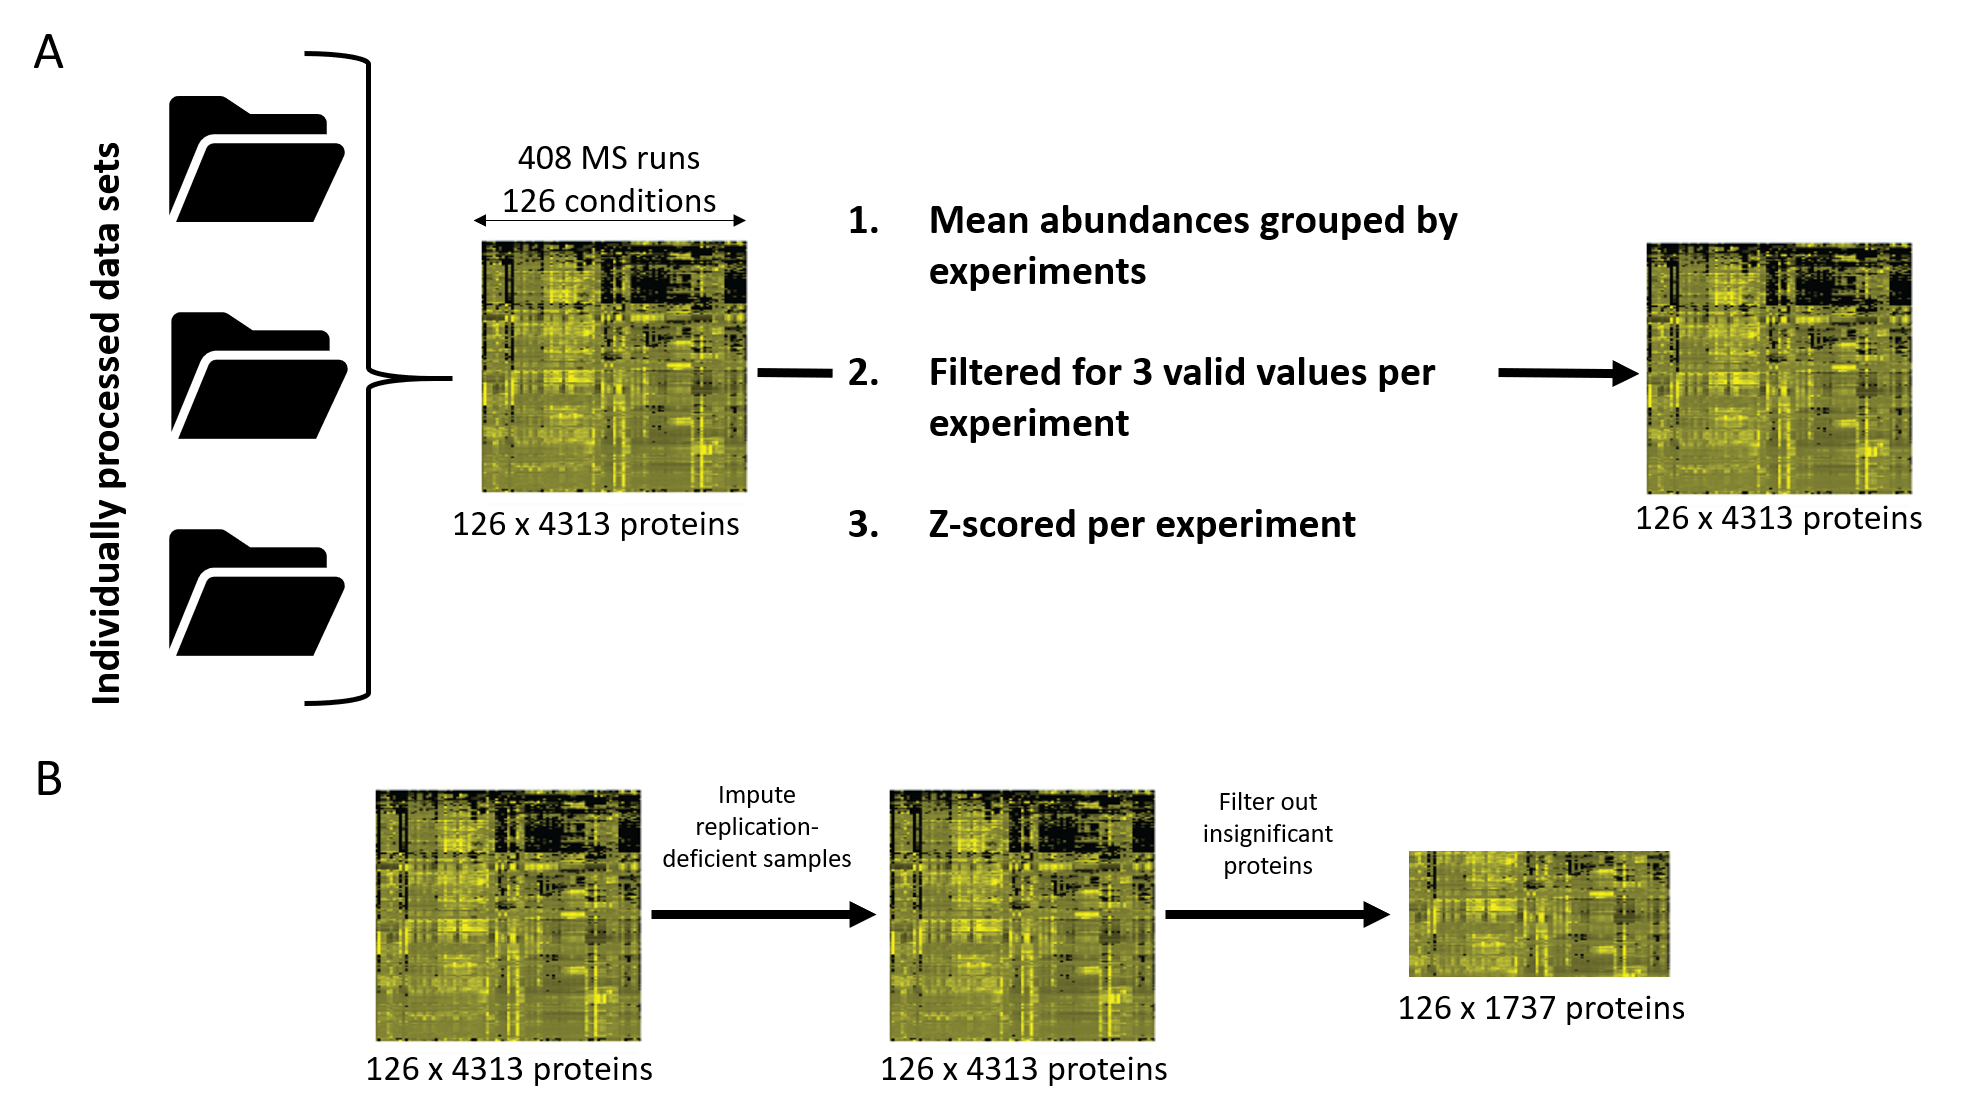
\includegraphics[width=\textwidth]{resources/images/Results/processing_step2.png}
    \caption[Processing of all datasets for visualization.]{\textbf{Processing of all datasets for visualization. }A) All individually processed data sets were combined into one large matrix containing abundances for 4313 proteins over 127 conditions collected in 408 mass spectrometry runs. The mean abundances per replicate where calculated and used to filter each protein for three valid values. This reduced the matrix to 1272 proteins over all conditions that where then Z-scored per experiment to normalize the abundance variation between them. This matrix was used as the input for all further computational methods. B) To improve performance of correlation and clustering algorithms the normalized matrix was further processed. First missing values in replication-deficient data sets were imputed utilizing a pseudo-random bootstrap method by replacing them with values from a normal distribution calculated from the rest of the abundances measured in the experiment. This imputed matrix was then filtered for proteins found to be significantly enriched under the investigated DNA lesions and already known and annotated DNA repair and replication proteins were added afterwards. The resulting matrix of 127 conditions with 1737 proteins each were used to construct new repair networks using Pearson correlation and Topological Overlap Measures.}
    \label{fig:processing}
\end{figure}

\begin{figure}[H]
    \centering
    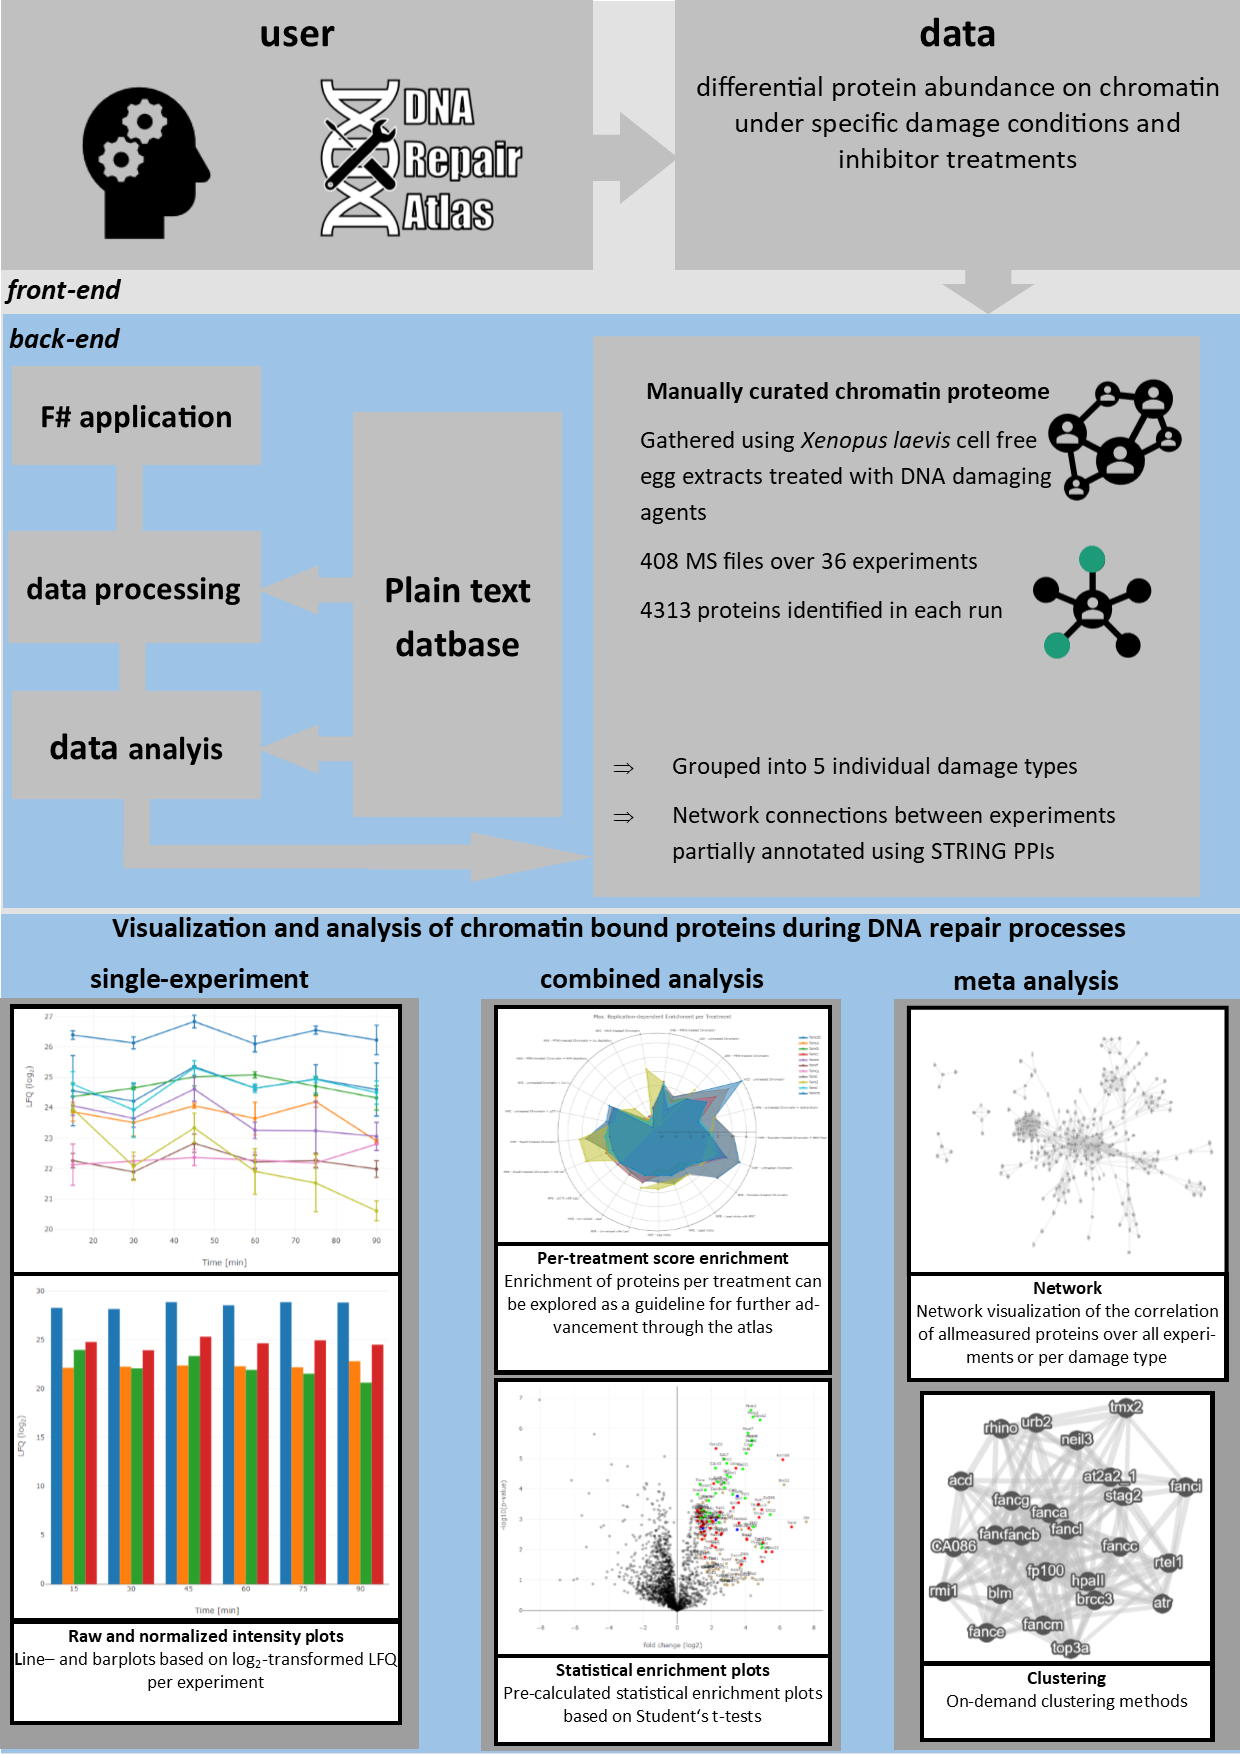
\includegraphics[width=\textwidth]{resources/images/Results/FlowChart.png}
\end{figure}
\newpage
\begin{center}
    \captionof{figure}[Setup and function of the DNA Repair Atlas]{\textbf{Setup and function of the DNA Repair Atlas.} A network representation of protein correlations based on their abundance on chromatin under different damaging conditions represents the central part of the DNA Repair Atlas. The measured \textit{Xenopus} proteins are mapped to the human homologue and annotated with links to protein/gene databases such as UniProt and GeneCard to improve access to the resource for new users. Due to restraints put on the project by the web-deployment method of choice all data needed for the processing and analysis are stored in a plain text database. Data processing and analysis is done on-demand after input from the user using scripts written in the functional programming language F\# running the \textit{back-end} of the resource. The user input as well as the information the \textit{back-end} returns are processed using JavaScript scripts at the \textit{front-end}. Several interfaces are implemented into the DNA Repair Atlas that allow easy access to the five main functions of the resource.}
    \label{fig:flowchart}
\end{center}
The user interacts with an HTML-based front-end deployed on a virtual machine hosted by the RHRK with 1 vCPU, 4 GB RAM and a 60 GB vDisk using Microsoft's Internet Information Service set up as a .NET application web-server. This front-end consists of different subpages with each of them focusing on one category of functions mentioned in Figure \ref{fig:flowchart}. Connecting this front-end to the back-end are scripts written in JavaScript that listen for pre-specified user-interactions and then send the information provided by the user to the back-end which in itself uses the library \textbf{Suave.IO} to listen for a specific set of information.
The back-end consists of a collection of modules written in the functional programming language F\# built mostly by Paul Menges during his master thesis \citep{Menges.2018} that are called using the information received by Suave.IO and return an output based on pre-defined permutations based on the input data. Streamlining and optimizing most of those modules and therefore maximize the user experience was one of this works main goals.\newpage
\subsection{Data (pre-)preprocessing}
\label{sec:processing}
A large part of this project was to optimize the pre-processing of the 408 input data sets based on proteomic analysis of chromatin bound proteins in \textit{Xenopus laevis} egg extracts. Due to the time span over which the data was collected and because it is advised if one wants to combine different collections of data in one large meta analysis we wanted to see how each group of experiments behaves in respect to all others. To do this the non-linear dimensionality reduction algorithm t-SNE was applied to a matrix of mean protein abundances over all time points and replicates of each experiment where columns represented experiments and rows defined protein abundances.\\ t-SNE itself uses the parameters \textit{dims}, \textit{theta} and \textit{perplexity} to alter the location of each data point on the map. \textit{Dims} can either be set to $2$ or $3$ and defines the dimensions one wants to reduce the high-dimensional data set to. In most biological circumstances two dimensions are sufficient to visualize relationships between data points. \textit{Theta} should always be set to $0.0$ for best results as it defines the error between different iterations the algorithm deems to be sufficient. Higher \textit{theta}-values improve computation times with a decrease in accuracy. The parameter \textit{perplexity} (loosely) defines how to balance  attention between local and global aspects of the input data and sort of "guesses" the number of close neighbours of each data point on the map. Due to this it always has to be smaller than the number of data points one wants to look at.\\
\begin{figure}[H]
    \centering
    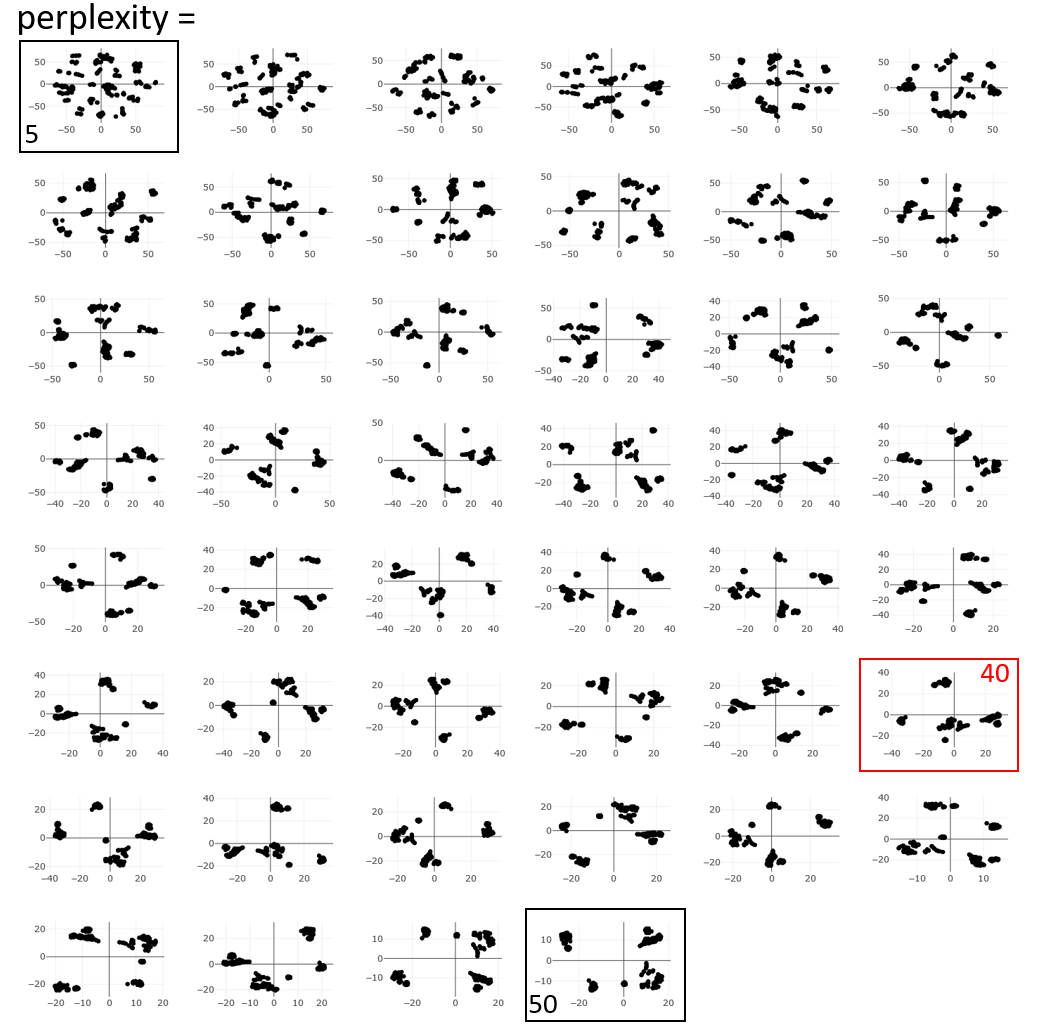
\includegraphics[width=\textwidth]{resources/images/Results/tSNE_opti.png}
    \caption[t-SNE Perplexity Optimization]{\textbf{t-SNE Perplexity Optimization. } A non-normalized matrix of mean protein abundances per experiment was filtered to include only the 1000 most prominent proteins based on their known ability to bind chromatin to lower computation times. \textit{theta} was set to 0.0 while \textit{perplexity} iterated from 5 to 50 in increments of 1. After comparing all resulting t-SNE maps we decided to continue with $perplexity = 40$ to avoid large indistinguishable groups.}
    \label{fig:tsneopti}
\end{figure}
To optimize the \textit{perplexity} for our use case we made the assumption that the result should show our data in two main and seven sub-groups that each represent the two different DNA templates, sperm chromatin and plasmid DNA, and the six different induced damages for each set of experiments. After applying t-SNE with perplexities between 5 and 50 to a pre-filtered data set we decided on \textit{dim} $= 2$, \textit{perplexity} $= 40$ and \textit{theta} $= 0.0$ for the final large scale t-SNE.\\
Those parameters resulted in the final map of all experiments shown below.
\begin{figure}[H]
    \centering
    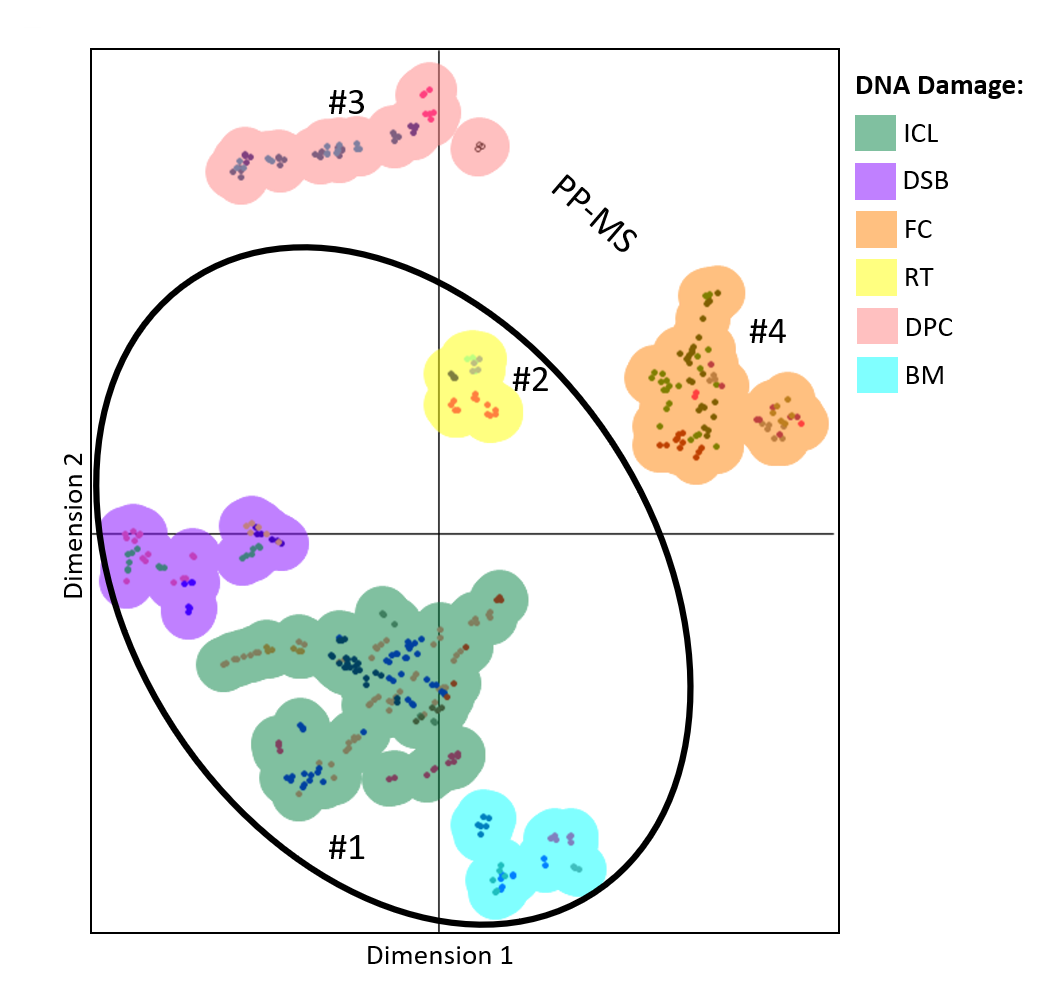
\includegraphics[width=.6\textwidth]{resources/images/Results/tSNE_map.png}
    \caption[Two-dimensional t-SNE map of all sets included in the Atlas]{\textbf{Two-dimensional t-SNE map of all sets included in the Atlas. }Non-normalized mean protein abundances for each experiment were used as an input for the t-SNE using the optimized parameters mentioned above. Colored clouds represent DNA lesions with: ICL = Interstrand Crosslink, DSB = Double-Strand Break, FC = Replication Fork Collapse, RT = Replication Termination, DPC = DNA-Protein Crosslink, BM = Base misincorporation. Data points included in the black ellipse represent experiment using sperm chromatin as the DNA while the others use plasmid vectors with defined lesions. Individual points inside the clouds each represent a single experiment and time point while their colors encode their chemical treatment (not of importance for this section). Numbers next to each group indicate the batch the sets were processed in due to their use in different publications.}
    \label{fig:tsnemap}
\end{figure}
Figure \ref{fig:tsnemap} shows a close relationship between all sets using sperm chromatin as a template (black ellipse) while still retaining closer grouping between each experiment series and the damage type induced respectively (cloud colors). Inside the larger clouds that represent experiment series each data point is individually colored in respect to its treatment. For example point colored pink always represent experiments using Geminin-treated extracts. Looking especially at the experiments colored in pink that are all deficient in DNA replication one can see them grouping away from replicating extracts of the same series while remaining in close vicinity.\\
As already mentioned some of the experiment sets were processed together in one processing session based on the publication they were used in (on the map indicated by \#1 through \#4). We previously expected this circumstance to have a large impact on the neighborhood on the t-SNE map but this does not seem to be the case. Neighborhood embedding seems to strongly depend on the DNA template and extract type used as well as the precise stage of replication and repair the experiment was focusing on. We can see this especially for processing group \#2 that uses sperm chromatin as a template but does not seem to embed closely to other experiments using the same substrate. This can be explained due to the experiment setup in general that was focused on investigating the termination of DNA replication specifically.  Due to the specific protein fingerprint of replication termination in comparison to all other sets and the synchronous nature of these experiments this group of experiments embeds distant from the other CHROMASS data sets and closer to the PP-MS sets were replication is more synchronized compared to CHROMASS. The PP-MS sets also embed far away from each other as expected due to the synchronized replication and the very strictly defined lesions present on the plasmid template.\\
From this preliminary data investigation using dimensionality reduction to build a neighborhood map of all experiments included in the atlas we can conclude that DNA template and lesions have a higher impact on the embedding of each experiment series. While still present, the effect of batch processing can be neglected once proper normalization steps are carried out for the whole collection of data sets. This is proves that the previous approach to visualizing DNA repair modules using a normalized pre-filtered network on the atlas was valid but could be improved by adding networks for each type of DNA lesion. Implementing such networks can, as will be discussed later in this thesis, noticeably improve the performance of clustering algorithms for the identification of functional DNA repair modules. t-SNE analysis showed that the sets are usable for the purposes of the DNA Repair Atlas but could be reprocessed together once the computational resources are available.\\
After validating that the data can be combined without batch effects inhibiting the creation of repair networks we moved on to prepare the data sets.\\\\
To enable filtering of significantly enriched proteins in later steps we used the combined matrix of protein abundances as an input for an R script utilizing Student's t-Tests with data dependent S\textsubscript{0} determination. This script used the package "samr" (https://CRAN.R-project.org/package=samr) to determine the S\textsubscript{0} for each comparison dependent on the data itself. This allowed us to automate the calculation of significance values for each protein regarding its enrichment based on predefined comparisons. The resulting p-values were stored in log\textsubscript{10} format and afterwards multiplied over all comparisons to obtain an arbitrary "Enrichment Score" over all experiments as well as for each DNA lesion separately. This score is used in the DRA in network styling as well as the base for the polar enrichment plot of each DNA lesion.\\  
As briefly described in Fig \ref{fig:processing} the individual data collections were combined into one matrix consisting of all 408 mass spectrometry runs over 126 conditions. In each run, a total of 4313 proteins could be detected whose mean abundances per replicate were calculated. For each experiment proteins with less than three valid values were filtered out.  This yielded a matrix with 1727 proteins over 126 conditions retaining time point information that was used as an input for the visualization functions of raw and normalized abundances for each experiment. As will later be shown the functions enabling this feature have been optimized to be more modular and user friendly.\\\\
To build the aforementioned networks for each type of DNA lesion this matrix was further processed to only include one value per protein for each experimental condition. Those conditions then were grouped by the DNA lesion repair they were used to investigate and split into separate matrices while keeping one ungrouped matrix containing all conditions. The "Enrichment Score" over all DNA lesions was filtered for all proteins with a higher score than the 90\textsuperscript{th} percentile to reduce the number of proteins to 1737. This list of proteins was deemed "interesting" and used to filter the individual DNA lesion matrices before applying WGCNA.\\


\subsection{Optimizing an interactive web application}
\label{sec:resource}
The development of an interactive web-resource based on mass spectrometry data is a complex endeavour that ideally starts with a concrete plan of action. This plan has to include the programming language of choice, the basic structure of the final website as well as the so called "handler" that connects back-end and front-end with each other. Additionally it has to be thought about how data is stored and whether or not the user has direct or indirect access to raw or pre-processed data. In our case we decided to build the back-end using the functional programming language \textbf{F\#} developed by Microsoft as part of their .NET Framework using the library \textbf{Suave.IO} to functionally create a webserver with an included link handler. The user front-end (from here on referenced as "website") was written and styled using the markup language HTML (\textit{Hyper Text Markup Language}) and the style sheet language CSS (\textit{Cascading Style Sheet}) in combination with the web-programming language JavaScript as a means to implement local program functionality on the website itself. JavaScript was chosen over alternatives such as the scripting language PHP (originally: \textit{Personal Home Page}; Now: \textit{Hypertext Preprocessor}) due to performance limitations of the hardware used to deploy the resource to the user. With JavaScript, everything except direct request to the back-end runs locally on the users machine where PHP is evaluated by the server itself. Details about this including parts of the code are included in subsection \ref{sec:resource}.\\

The general structure of the resource can be seen in Figure \ref{fig:flowchart}. This flowchart shows the setup of the DNA Repair Atlas as well as the methods used to store data and an overview of the functions provided to the user to explore said data. The core functionalities were only adapted to challenges that arose during a test phase of the DRA and new methods were applied where necessary.\\

The first addition was a feature we call "Protein Search" with which the user can send a list of proteins of interest to the server and the server compares it to a list of registered proteins. If the proteins or any synonyms are found in the plain text database the server returns a list of enrichment scores which are plotted as polar plots using Plotly.js. The scores plotted are based on the filtered enrichment score matrix that only contains the 1737 most significantly enriched proteins over all datasets. The DRA itself offers the possibility to mine data for all 4313 proteins detected in the raw matrix with other features that will be explained later.
\lstset{language=FSharp}
\begin{lstlisting}
let rec radialData 
    (metaData:(string*float*float*float*float*float*float)list) (poi:string*string) =
        match metaData with
        | [] -> []
        | ((prot,all,dpc,dsb,fc,icl,rt) :: rest) when prot = (fst poi) ->
          (prot,dpc,dsb,fc,icl,rt) :: radialData rest poi
        | (_ :: rest) -> radialData rest poi
\end{lstlisting}
This function is especially useful for new users of the atlas that are are interested in the list of proteins included in it. Additionally it is useful to check if a protein one is interested in is significantly enriched in one of the DNA lesion sets included in the DRA. If one is for example interested in the enrichment of the Fanconi anemia core Complex it is possible to plot all subunits at once.
\begin{figure}[H]
    \centering
    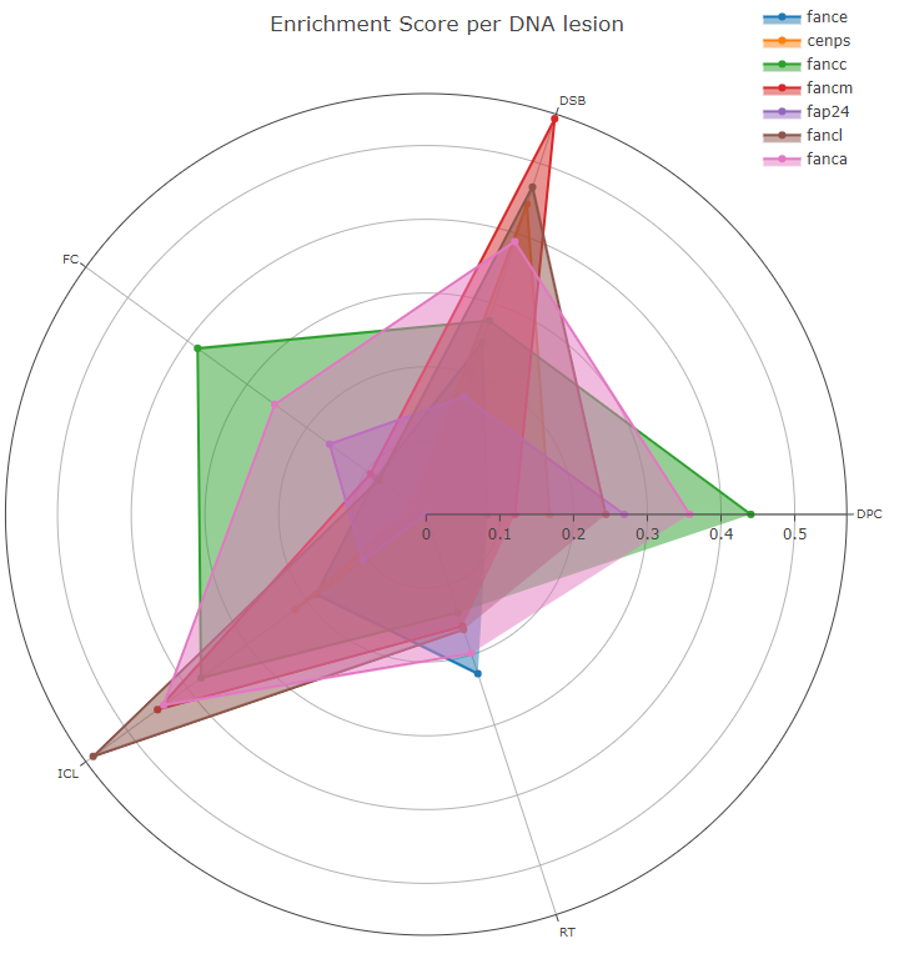
\includegraphics[width=0.6\textwidth]{resources/images/Results/fanc_enrichment.png}
    \caption[Relative enrichment of Fanconi Core Complex subunits]{\textbf{Relative enrichment of Fanconi Core Complex subunits. }Enrichment scores for each subunit of the Fanconi Core Complex included in the filtered list of enriched factors. Included are only those subunits that are enriched over all data sets but the scores are specific to each DNA lesion.}
    \label{fig:fanc_enrichment}
\end{figure}
The figure shows that subunits of the Fanconi Core complex seem to be enriched on chromatin in experiments investigating Interstrand Crosslinks and Doublestrand Breaks but fancc and fanca seem to be slightly enriched in DNA-Protein Crosslink and Replication Termination experiments. This could be an indication of homologueous recombination dependent DPC repair being mediated by the Fanconi anemia pathway in higher eukaryotes \citep{Stingele.2015}. Generally this feature of the DNA Repair Atlas gives the user a good idea of what to expect from the Atlas itself. It provides an overview of which DNA repair pathways can be investigated and how well certain parts of the proteome are represented.
\newpage

The next more detailed part of the DRA is a feature that lets the user plot intensity data over time for each experiment and all 4313 proteins either in LFQ or in normalized LFQ (z-scored) values.\\
Previously, this module was built to only work with the specific plain text database where rows represented individual proteins and each column represented a single proteomic data file. The function written to extract data from this set based on the user input consisting of an experiment is shown below.
\lstset{language=FSharp}
\begin{lstlisting}
let chooseExperiment (exp:string) =
    match exp with //matches the input experiments with pre-defined keys in the database
    |"Key" -> let Exp_Time_1 = 
                    [for row in textDataBase.Rows -> row.Exp_Time_1]
                    |> Seq.ofList 
                    |> Seq.zip miscData
    //and uses FSharp.Data to extract matching intensities per timepoint
              let Exp_Time_2 = 
                    [for row in textDataBase.Rows -> row.Exp_Time_2] 
                    |> Seq.ofList 
                    |> Seq.zip miscData
    //to finally merge to a sequence of two tupled lists containing intensities and time
             seq[Exp_Time_1;Exp_Time_2],["1";"2"]
                   
    |"" -> seq[],[]
\end{lstlisting}
Put simply, this function matches the experiment chosen by the user with \textit{hard coded} experiments in the database, extracts every row of the column representing this experiment and then merges it with a list of proteins defined elsewhere. In the context of the resource this function is called within another function that gets the experiment and a list of proteins of interest as an input and that outputs data in the format the front-end needs to plot a time course or protein intensities for the selected experiment and treatment. To improve on this function design we looked at the input file and how data is extracted from it. Noticeable was that each time a new data set was added to the collection there were two locations in the code that had to be adapted to fit the new input structure. Not only had the HTML document to be updated but also the matching function in the back-end. We came to the conclusion that it would be easier to store the data in such a way that new data sets could be added without the need to update most of the code. To achieve this we implemented a function that takes a plain text file, an experiment, a treatment condition and a list of proteins as its input. The list of proteins is fed to the function in string format to simplify the interaction between the back- and front-end.
\newpage

\lstset{language=FSharp}
\begin{lstlisting}
let searchForProteinData (data:CsvFile<CsvRow>) (expIn:string) (protList:string) (treatIn:string) =
    let lfqValueSeq = 
        let proteins = data.Headers.Value |> Array.tail |> Seq.ofArray
        seq[for i in (addedNames protList) -> proteins |> Seq.filter (fun x -> x.StartsWith(fst i))]
        |> Seq.concat
        |> Seq.map (fun p -> proteins 
                             |> (fun _ -> data.Rows 
                                          |> Seq.map (fun y -> try float (y.GetColumn p) with | :? Collections.Generic.KeyNotFoundException -> nan))
                             |> Seq.zip [for row in data.Rows ->
                                            int (row.GetColumn "FILE_ID")],p)             
    let filteredMeta = 
        let filtered = (metaDataParse.Filter (fun x -> String.Equals((x.GetColumn "Treatment"), treatIn) )).Filter ( fun x -> String.Equals((x.GetColumn "Experiment Series"), expIn))
        seq[for row in filtered.Rows ->
                int (row.GetColumn "FILE_ID"), row.GetColumn "Treatment", row.GetColumn "Experiment Series", row.GetColumn "Time"]
    let treatment = filteredMeta |> Seq.map (fun (_,treat,_,_) -> treat) |> Seq.head
    let inter = 
        filteredMeta 
        |> Seq.collect (fun (metaID,_,_,time) -> (lfqValueSeq |> Seq.map (fun (valueSeq,protName) -> (valueSeq |> Seq.tryFind ( fun (lfqID,_) -> lfqID = metaID),protName,time))))
        |> Seq.map (fun (valOpt,protName,time) -> match valOpt with
                                                  | Some x -> (snd x), protName,time
                                                  | None -> nan,protName,time)
    inter
    |> Seq.filter (fun (lfq,_,_) -> (Double.IsNaN >> not) lfq )                      
    |> Seq.groupBy (fun (_,y,z) -> y,z) 
    |> Seq.map (fun (groupName,myGroup) -> groupName,(myGroup |> Seq.map ( fun (lfq,_,time) -> lfq,time)))   
    |> Seq.map (fun ((p,t),x) -> (p,t),(List.ofSeq x |> List.unzip))
    |> Seq.map (fun ((p,t),(vL,_)) -> p,vL,t,(List.averageBy float vL),(sDev vL))
    |> Seq.groupBy (fun (p,_,_,_,_) -> p)
    |> Seq.map (fun (groups,data) -> groups,data |> Seq.map ( fun (_,_,t,vm,e) -> (vm,e,t) ) |> List.ofSeq |> List.unzip3)
    |> Seq.map (fun (n,(y,e,x)) -> (n,treatment,(y,e,x)))
    |> Seq.sortByDescending (fun (prot,_,(_,_,_)) -> prot)
\end{lstlisting}
Note that in this case the data is split into two files with one containing meta information and the other the LFQ intensities. The two files are matched using unique IDs. This format was chosen to make it easier to maintain the meta data and make changes on the fly without risking to alter the LFQ intensity file. In general applying this function results in the same output as the function mentioned above, but the mechanism by which it works allows easier maintenance.\\
Additionally this change gave way to a dynamically filled drop-down menu on the front-end. Each time an experiment series is selected (see Figure \ref{fig:dropdown_plotting}) the drop-down menu for selecting the experimental condition is updated to show all valid options. To do this the front-end request a JSON string containing a map of experiment series and their valid conditions anytime the experiment selector is changed. 
\begin{figure}[H]
    \centering
    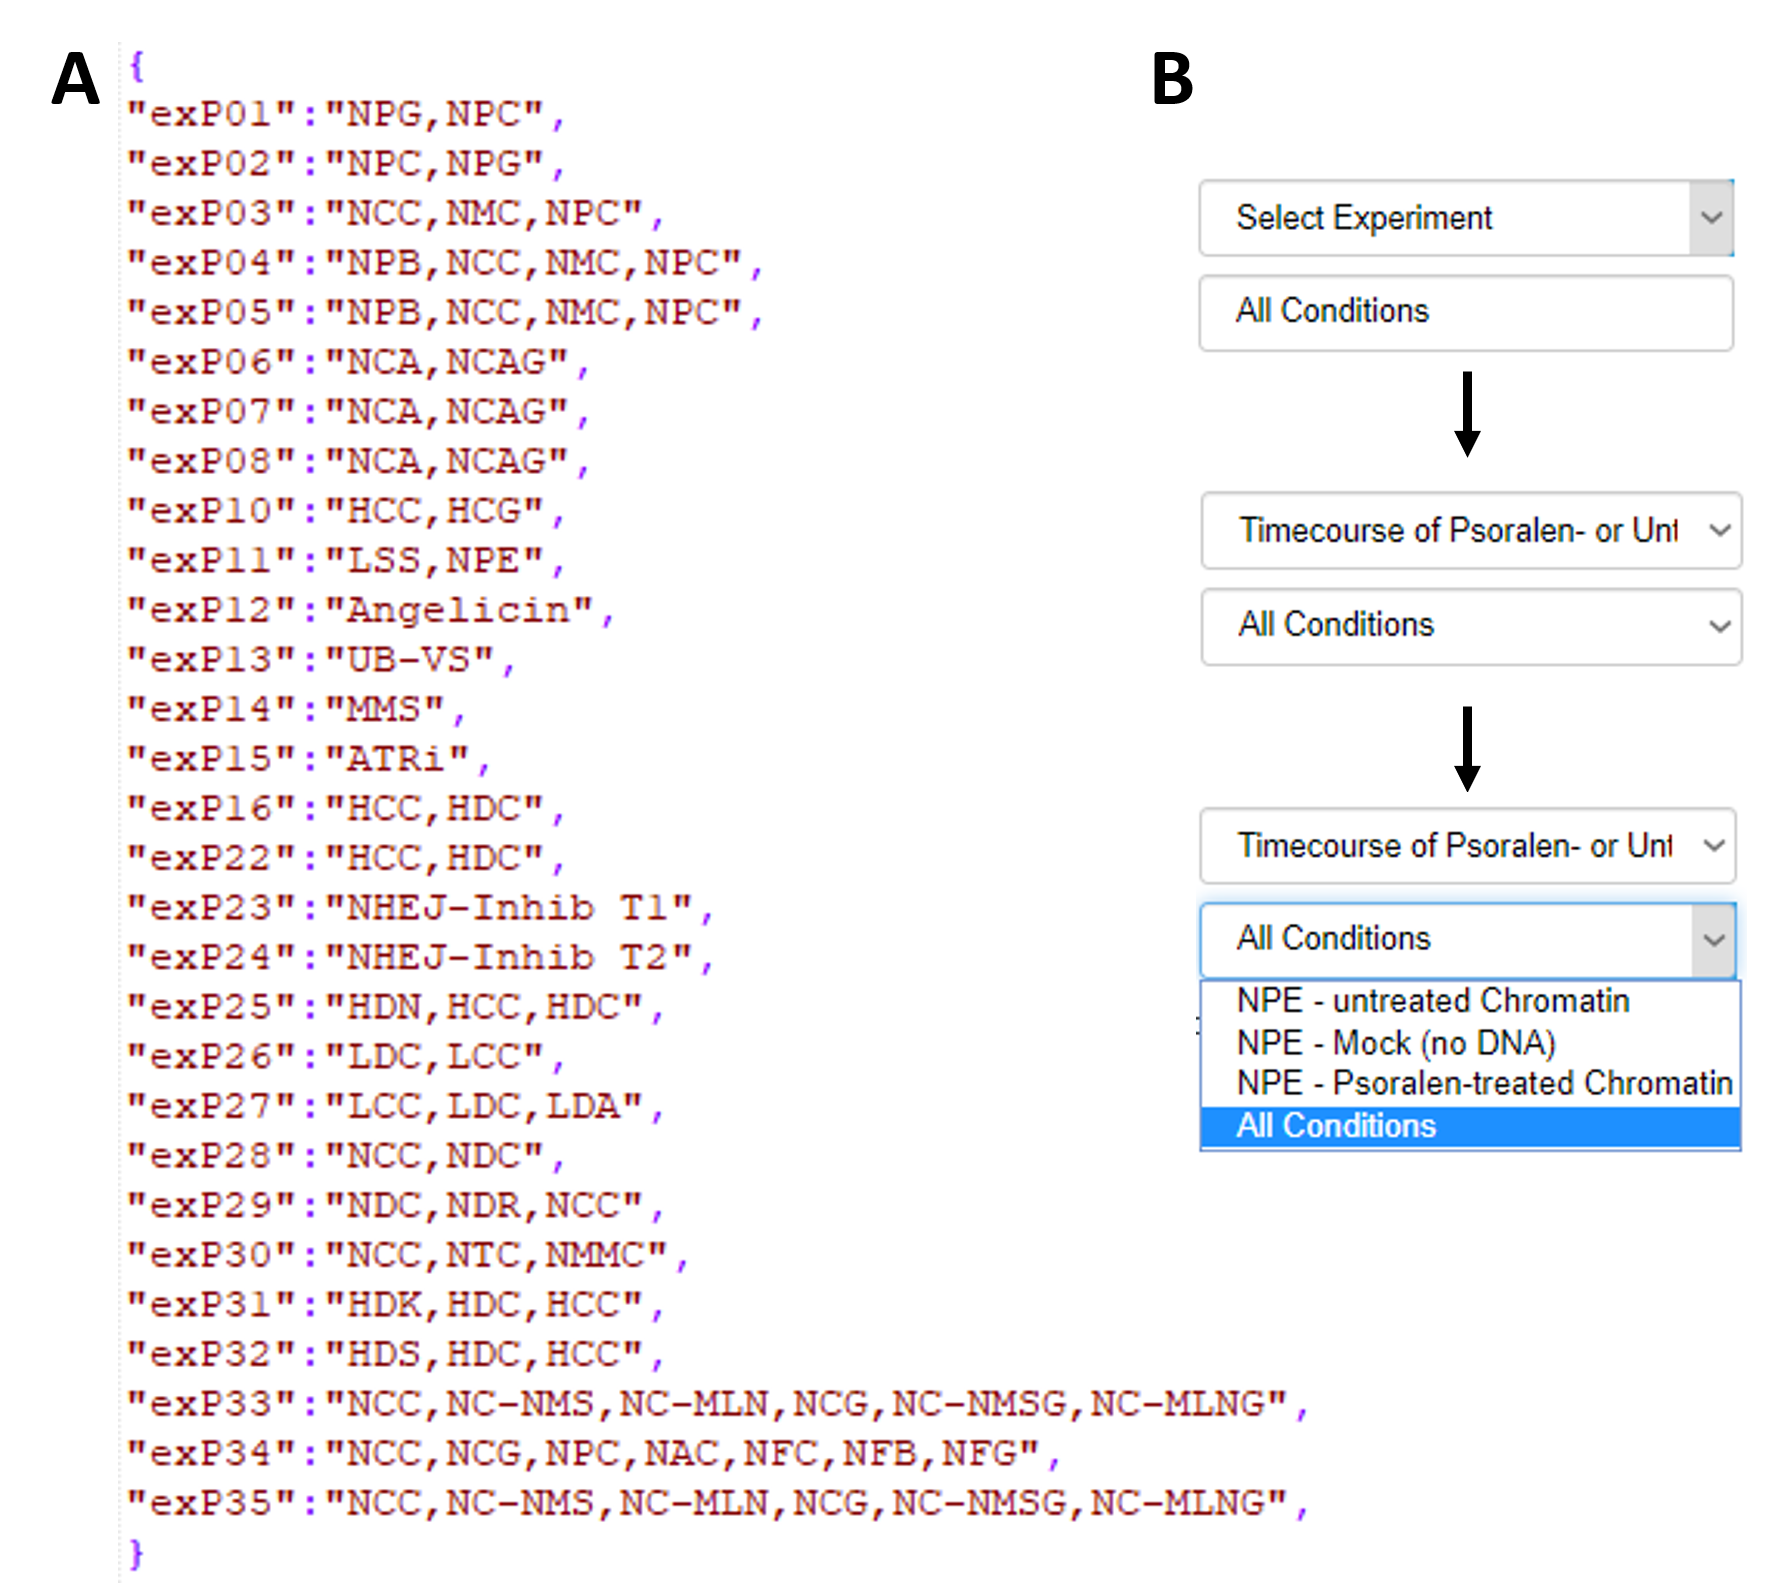
\includegraphics[width=.7\textwidth]{resources/images/Results/dropdown_plotting.png}
    \caption[Filling a Drop-Down menu with JSON data]{\textbf{Filling a Drop-Down menu with JSON data. }A) Illsutarted is the JSON string the front-end request each time the experiment selector is changed. The JSON string represents a map that contains keys representing individual experiments that are matched via a JavaScript function and respective values that are used to fill the second dropdown menu dynamically. B) An overview of the drop-down menus used to select an experiment and the dynamically filled treatment.}
    \label{fig:dropdown_plotting}
\end{figure}
The dynamic addition and removal of drop-down options given the described JSON map is handled via the following JavaScript function. This function uses a switch-case statement to match key values of the JSON map requested from the back-end to extract their respective values. It then uses another switch-case statement to match the three-letter treatment codes with human readable treatment descriptions that are added to the treatment selection drop-down menu.\\
\newpage
\lstset{language=htmlcssjs}
\begin{lstlisting}
function updateTreatments() {
    var $dropdown = $("#exp");
    $.getJSON("/expList", function (expdata) {
        var key = $dropdown.val();
        var vals = [];
        //matches JSON string keys with current experiment drop-down value and returns corresponding treatment codes
        switch (key) {
            case 'EXP01':
                vals = expdata.exP01.split(',');
                break;
            case 'EXP02':
                vals = expdata.exP02.split(',');
                break;
            case 'EXP03':
                vals = expdata.exP03.split(',');
                break;
            ...
            case 'base':
                vals = ['<option>Can not switch to</option>'];
        }
        //matches the extracted treament codes from the JSON string and returns drop-down items
        var $treatChoice = $("#treat");
        $treatChoice.empty();
        $.each(vals, function (index, value) {
            switch (value) {
                case 'NCC':
                    $treatChoice.append('<option value = "' + value + '">NPE - untreated Chromatin</option>');
                    break;
                case 'NMC':
                    $treatChoice.append('<option value = "' + value + '">NPE - Mock (no DNA)</option>');
                    break;
                case 'NPC':
                    $treatChoice.append('<option value = "' + value + '">NPE - Psoralen-treated Chromatin</option>');
                    break;
                case 'NPG':
                    $treatChoice.append('<option value = "' + value + '">NPE - Psoralen-treated Chromatin + Geminin</option>');
                    break;
                ...
                default:
                    $treatChoice.append('<option value = "' + value + '">' + value + '</option>');
                    break;
            }
        });
        $treatChoice.append('<option value ="' + vals + '" selected>All Conditions</option>');
    });
}; 
\end{lstlisting}
The last version of the DRA included only the option to use specific predefined protein names as an input for the plotting- and search functions. This has been updated to include the UniProtIDs for each human homologue of the included proteins as well as major Gene Ontology (GO) codes (Cellular Compartment = CC; Biological Process = BP; Molecular Function = MF). This gives the user the opportunity to input a certain GO-term and plot all proteins in the database that are annotated with that term. For example if a user is interested in the changes of protein abundance on Psoralen-treated chromatin over time for the Fanconi anemia complex proteins it is not necessary to type each subunit into the input field but the GO term would be sufficient.
\begin{figure}[H]
    \centering
    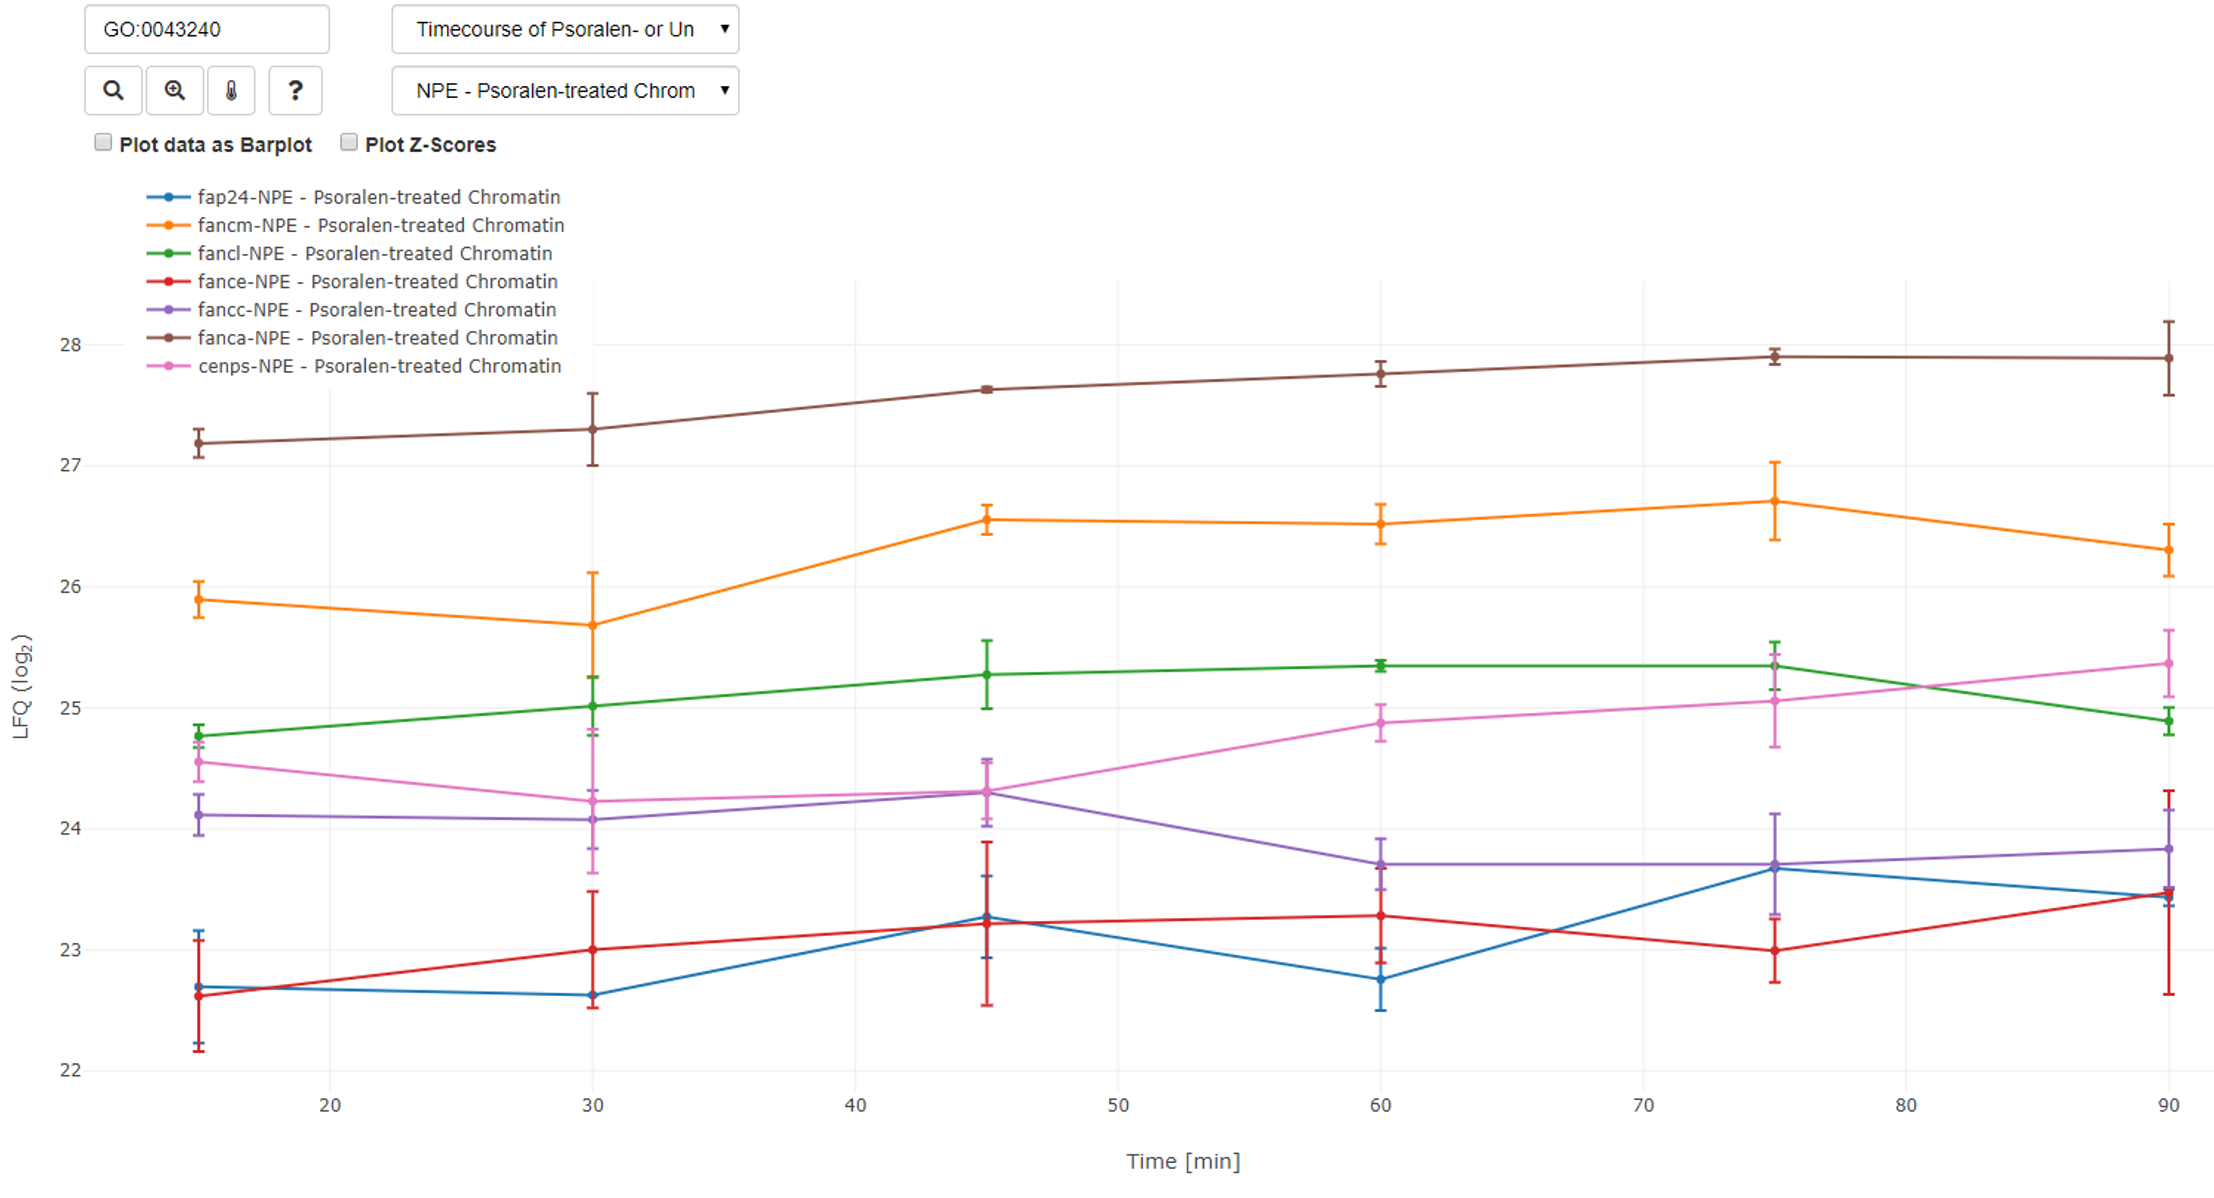
\includegraphics[width=\textwidth]{resources/images/Results/fanc_plottingPso.png}
    \caption[Supplementary Intensity Plots]{\textbf{Supplementary Intensity Plots. }The DRA features the option to plot the changes in abundance on chromatin for each included protein, experiment and experimental condition. The user has the option to either plot line- or bar plots over time given the standard deviation as error bars per time point as well as normalized (z-scored) intensities without error bars.}
    \label{fig:fanc_plotting}
\end{figure}
This feature has been implemented globally so that it functions with all basic input fields on the DRA. Functionally the back-end stores all annotation data for each protein in a large plain text table with the structure shown in Figure \ref{fig:annotation} and applies a function called \textit{addedNames} to every text input made by the user.
\newpage
\begin{wrapfigure}{l}{0.4\textwidth}
    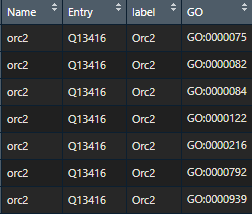
\includegraphics[width=0.36\textwidth]{resources/images/Results/annotation.PNG}
    \caption[Small excerpt from the annotation table used for data mining]{\textbf{Small excerpt from the annotation table used for data mining. }Shown is a list of additional names for the Origin Recognition Complex subunit orc2. Note that each row represents a single given combination of all possible inputs that result in orc2 being used as a query protein. Available are a multitude of GO terms (GO) as well as the gene name (Name), an alternative gene name (label), human homologue UniProtID (Entry).}
    \label{fig:annotation}
\end{wrapfigure}
\textit{addedNames} takes the user input string which can be a single protein of interest, a list of proteins or a GO term and splits it into a Sequence of strings. Each element of this sequence is then matched against a protein annotation file containing multiple entries for each protein present in the database based on ever single possible GO term and UniProtID for that protein. If a match is found, the function returns a list of proteins with identification values that match the ones used in the plain text data base of the DRA, effectively translating known alternative names and IDs to usable protein names. As this function can be called inside any other function extracting information for a protein from the data base, we've implemented a way to use multiple identification systems with the DRA that can be easily adapted once new proteins get added or more identifiers are needed. Especially useful is the inclusion of GO terms due to their ease of use and the possibility to use them as an easier input for clustering algorithms using multiple proteins as their input - such as the Diffusion algorithm implemented in the DRA by \cite{Menges.2018} (see Section \ref{sec:diffusion}).
\lstset{language=FSharp}
\begin{lstlisting}
let addedNames (inString:string) =
    inString.Split [|',';';'|] |> Array.filter (String.IsNullOrWhiteSpace >> not) |> Array.map ( fun x -> x.Trim()) |> Seq.ofArray
    |> Seq.collect ( fun inputProt -> 
                     additionalNames 
                     |> List.map ( fun x -> 
                                   match x with
                                   | (a,_,_,_) when String.Equals (a,inputProt) -> a,inputProt 
                                   | (a,b,_,_) when String.Equals (b,inputProt) -> a,inputProt 
                                   | (a,_,c,_) when String.Equals (c,inputProt) -> a,inputProt
                                   | (a,_,_,d) when String.Equals (d,inputProt) -> a,inputProt
                                   | _ -> inputProt,inputProt ) )
    |> Seq.distinctBy fst
    |> ( fun x -> if (inString.StartsWith "GO:") || (inString.StartsWith "EC:") then
                    x |> Seq.filter ( fun (a,b) -> not (String.Equals (a,b)) )
                  else
                    x)
    |> Seq.filter ( fun (a,b) -> (String.IsNullOrWhiteSpace >> not) a )
    |> List.ofSeq
\end{lstlisting}\newpage
\begin{figure}[H]
    \centering
    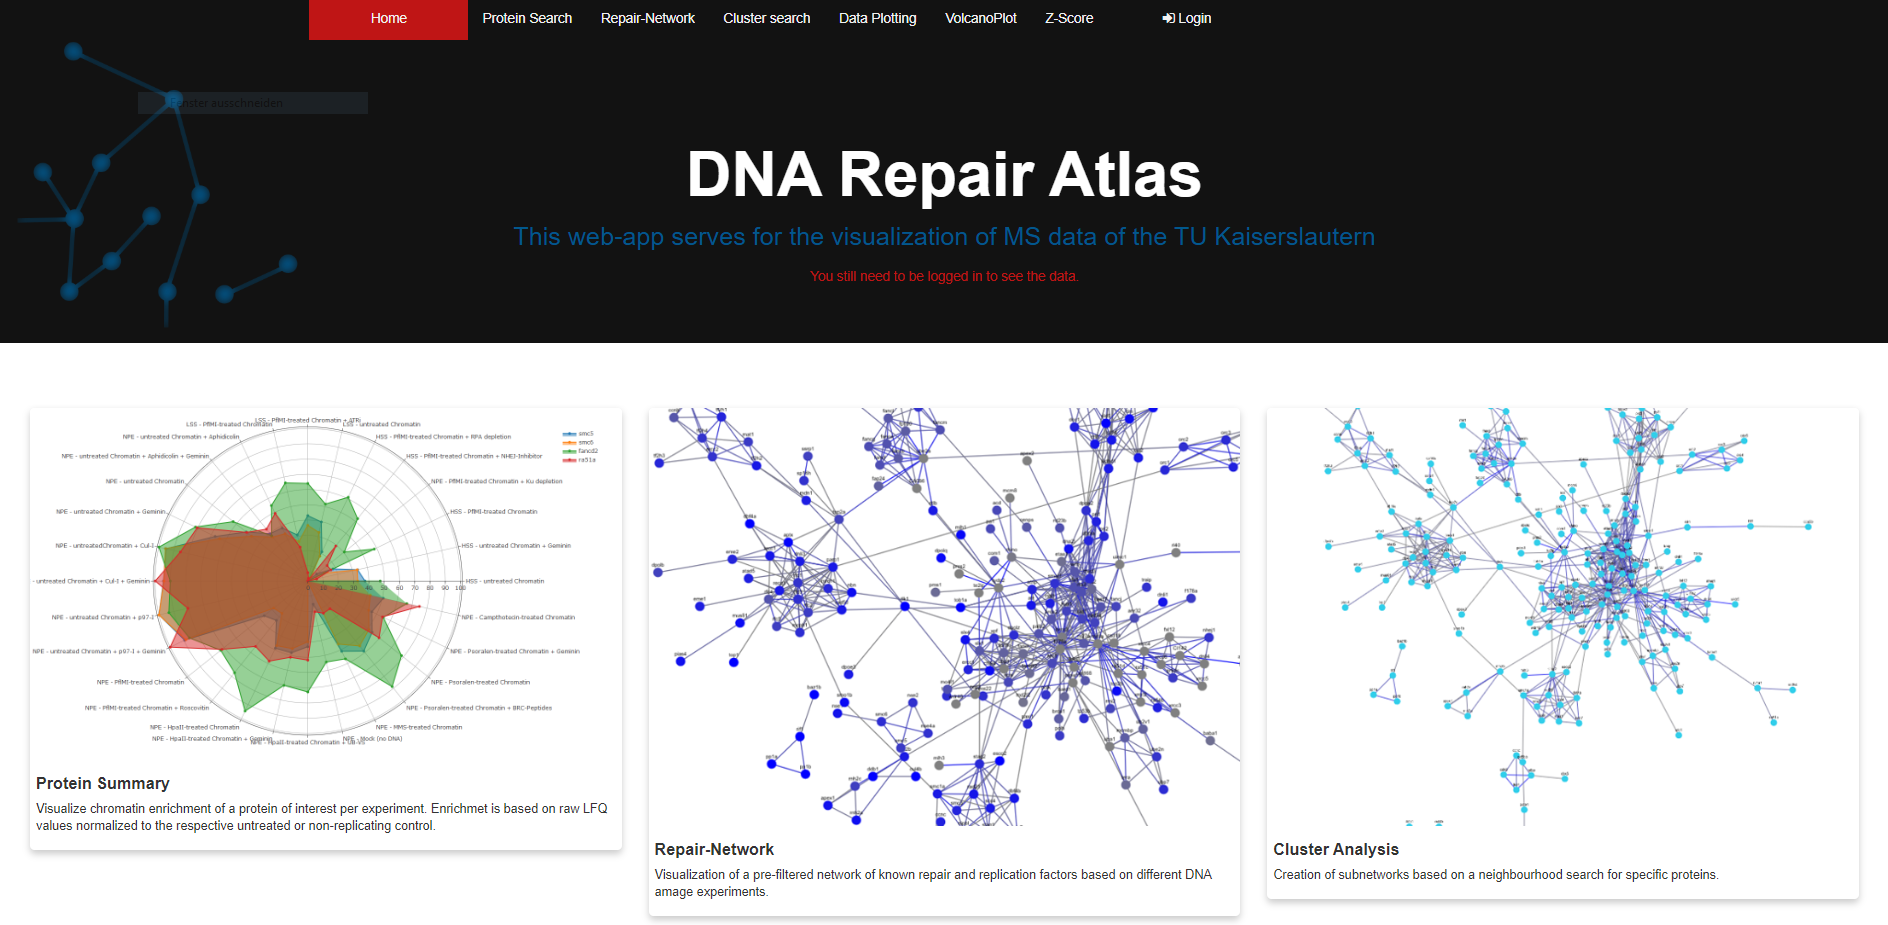
\includegraphics[width=\textwidth]{resources/images/Results/home.PNG}
    \caption[Screenshot of the starting page of the DNA Repair Atlas]{\textbf{Screenshot of the starting page of the DNA Repair Atlas. }Shown is a screenshot of the starting page with the visual represenations of all major functions as well as descriptive texts for each of the sub-pages.}
    \label{fig:home}
\end{figure}
In addition to some changes on a functional level the design of the DRA has been updated to improve the user experience. The starting page now shows a visual representation of all included functionalities as well as descriptive texts for each major sub-page.\\
For the remainder of this thesis we will focus on the \textbf{Cluster Search} starting with how the networks that can be plotted were created and what they can be used for.

\subsubsection{Constructing DNA lesion specific networks using modified WGCNA}
\label{sec:netprocessing}
Filtered matrices for each DNA lesion were transposed so that columns represented proteins. Due to the low number of experiment sets included in the collection for Base Misincorporations we omitted this set from the network creation. The Pearson correlation coefficient for each column was then calculated using the R package "Hmisc" (https://CRAN.R-project.org/package=Hmisc) that also reports the significance of each correlation value. The correlation matrices were then flattened to obtain lists of the format shown in Table \ref{tab:corrFlat}.
\begin{center}
 \begin{tabular}{c c c c} 
 Protein A & Protein B & Correlation & p-value \\ [0.5ex] 
 \hline
 acbp4 & abcf1 & 0.5645 & 0.03 \\ 
 aldoa & actc & 0.9001 & 4.8e-10
 \label{tab:corrFlat}
\end{tabular}
\end{center}
Every correlation coefficient with a p-value below 0.01 was then filtered out and anti-correlations were removed because they were not used in network construction. From the columns "Protein A", "Protein B" and "Correlation" we reconstructed a correlation matrix and a sigmoid adjacency function included in the R package WGCNA  \citep{PeterLangfelder.2008} with $mu=0.91$ and $alpha = 37$ to apply a soft-threshold to the correlation matrix. The result of this was used to compute the Topological Overlap Measure (TOM) that defines co-expression or in our case co-binding patterns using a geometric measure based on a similarity matrix.\\
The calculated TOM and Adjacency matrices were flattened and merged together to form lists of adjacencies (SIM) and TOM values for each protein-protein relationship. Those lists can be considered to be edge lists that are used to create the network on the DRA.
\begin{center}
 \begin{tabular}{c c c c} 
 Source & Target & SIM & TOM \\ [0.5ex] 
 \hline
anxa5 & aimp1 & 0.7932 & 0.1133\\
anxa5 & aldoa & 0.9723 & 0.6644
  \label{tab:edgeLists}
\end{tabular}
\end{center}
They contain a column that specifies the Source node, a column that denotes the Target node and one column for Pearson's correlation coefficient and the Topological Overlap Measure. How the F\# back-end creates a network from this edge list will be mentioned in Section \ref{sec:resource}. The difference between TOM and correlation networks can be seen below in Figure \ref{fig:tomvscor}. To ensure that TOM is a measure that can be applied to our data we had to check if the networks that are created from it can be considered "scale free". In scale free networks the node degree, meaning the number of direct neighbours of each node, follows a power distribution.
\begin{equation}
    P(k) \sim k^{-y}
\end{equation}\\
Checking if our TOM matrices follow this rule and can be considered scale free was done by plotting the fraction of nodes of a certain degree (P\textsubscript{k}) against the degree k on a logarithmic scale for the networks of each major DNA lesion.
\begin{figure}[H]
    \centering
    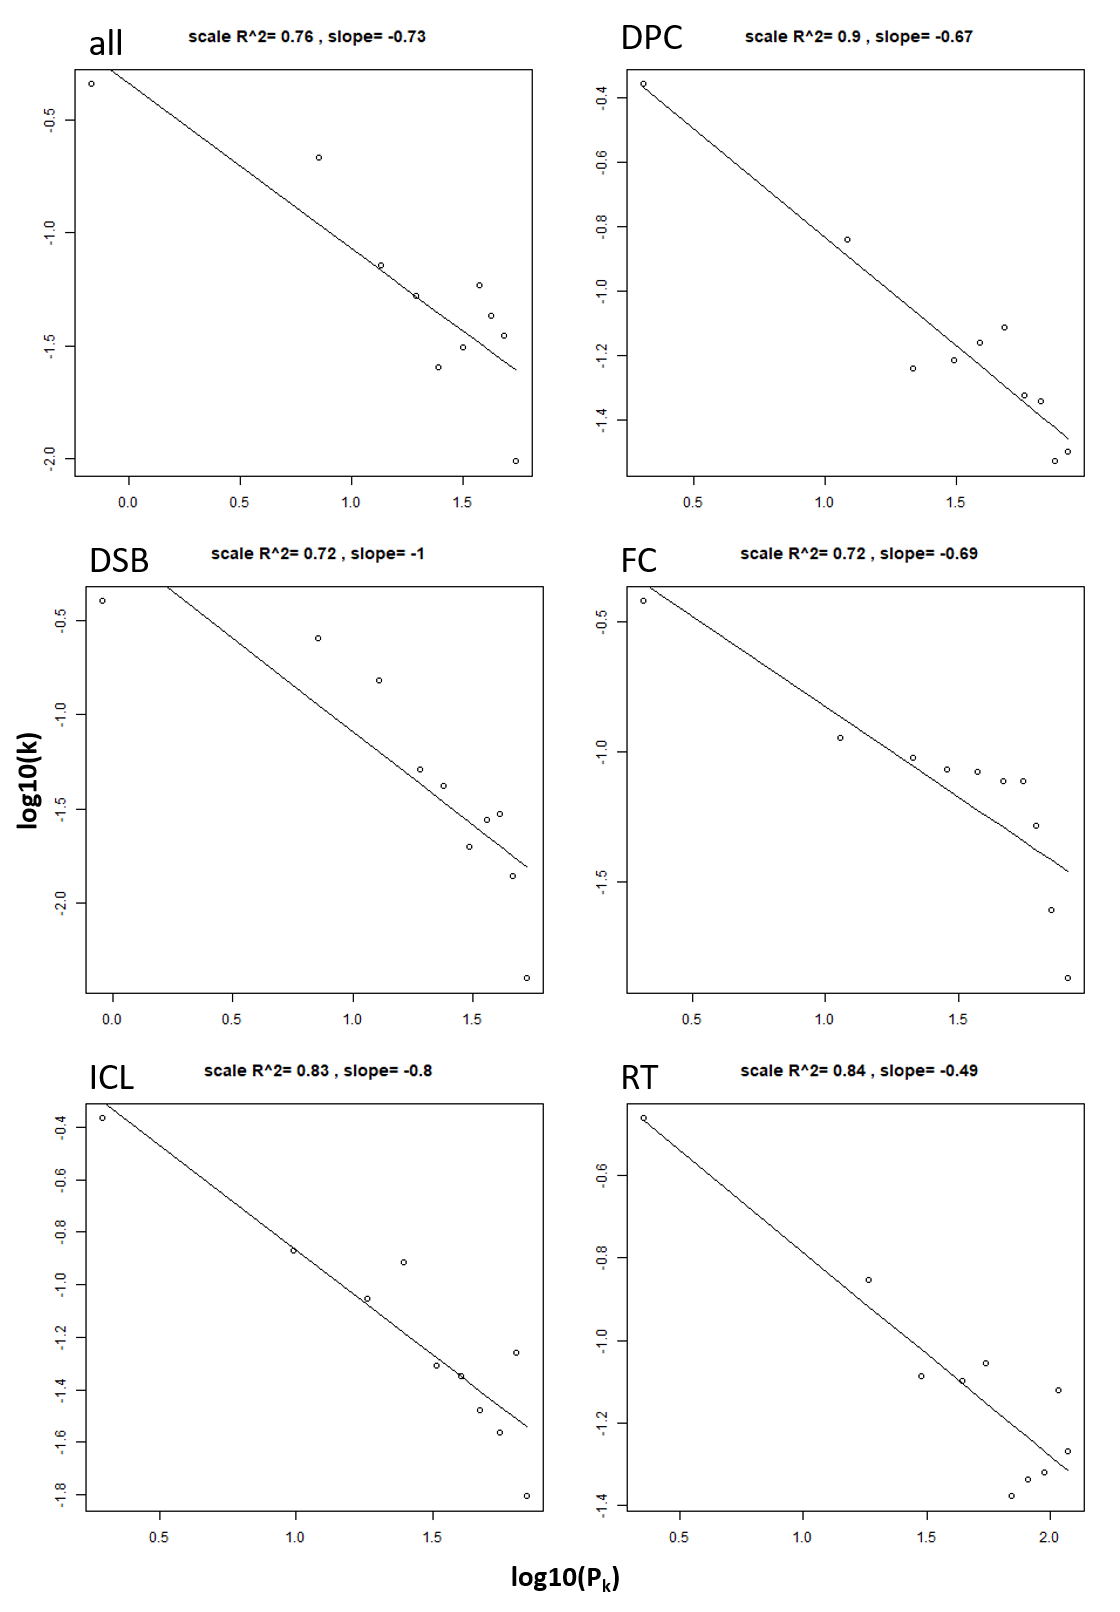
\includegraphics[width=\textwidth]{resources/images/Results/scaleFreePage.png}
    \caption[Scale free plots for all newly constructed TOM networks]{\textbf{Scale free plots for all newly constructed TOM networks. }Plotting of scale free plots was done using the a built-in function of the WGCNA package and native R methods.}
    \label{fig:scaleFreeness}
\end{figure}
If a network is scale free its node degree distribution should follow a power law which is indicated in these logarithmic plots as a linear model. The slope of this model is not really relevant for our observation of scale-freeness but the regression coefficient value shown above each plot indicates how well the networks follow the power law. Networks with an regression coefficient of above 0.6 can be considered scale free in the biological context due to real scale-freeness being very rare in real life data \citep{Broido.2019}. Given these thresholds all of our TOM networks can be considered to be scale free (see Figure \ref{fig:scaleFreeness}). Networks that do not fit this criterion can of course still be used for clustering algorithms but can yield less reliable results because they do not follow the small world principle of sufficient connectivity between all network nodes.
\begin{figure}[H]
    \centering
    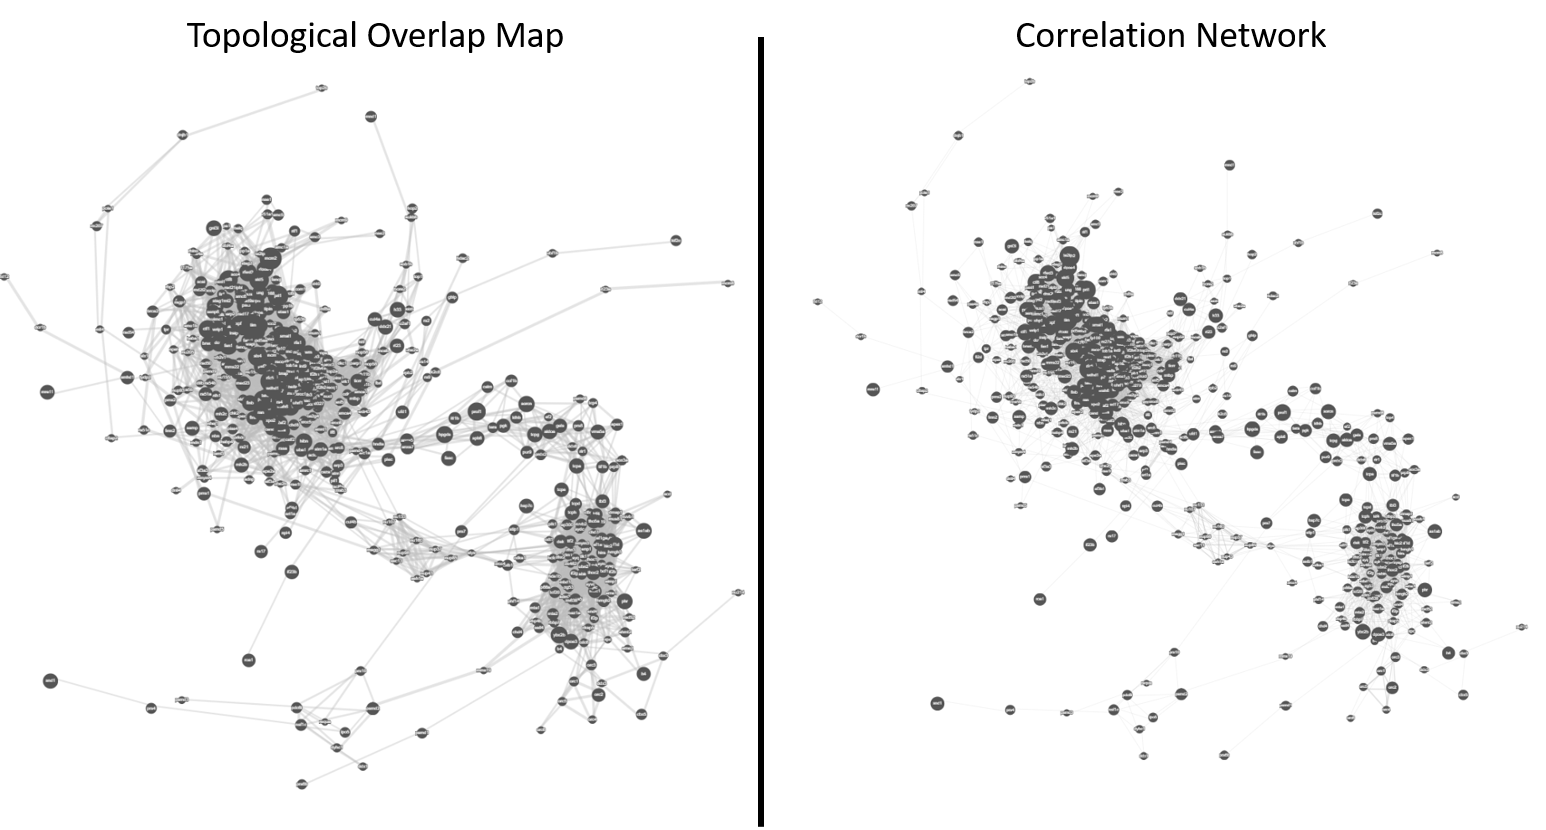
\includegraphics[width=\textwidth]{resources/images/Results/sim_tom_icl.png}
    \caption[Comparison of a Pearson Correlation Network and the respective Topological Overlap Map]{\textbf{Comparison of a Pearson Correlation Network and the respective Topological Overlap Map. } The topological overlap map and correlation network for all ICL sets were plotted next to each other. One has to note that the edges of the correlation network are unfiltered while the TOM is filtered using a soft threshold defined as $theta = 0.7 * EdgeWeight_{max}$. These two networks exist to visualize the difference between TOM and correlation and are based on a filtered protein list. They do not represent the networks that can be browsed on the DRA itself.}
    \label{fig:tomvscor}
\end{figure}
\newpage
Given the filtered nature of the TOM compared to the correlation network one can say that TOM represents protein co-regulation on a broader scale. If the correlation network were to be filtered by the same criteria, only about 50 nodes would remain in the final network. This is of course not sufficient for effective clustering and especially not useful for the identification of novel co-regulations or interactions. Generally it seems that TOMs expand the correlation network to a point where normally removed nodes are still included. Therefore it retains more information about the actual co-regulations of repair proteins. The implemented clustering algorithms of the DRA work on unfiltered versions of each networks to maximize the available data and greatly improve the ability to mine data. Due to the mentioned reasons we did not include raw correlation or adjacency networks except for the already existing curated networks.\\
To improve 
The networks constructed were then further processed depending on the needs of the user of the DRA. They can either be plotted and browsed or used as a base for Nearest Neighbor Clustering or a Diffusion algorithm to find functional clusters within the network as shown in Figure \ref{fig:co-expression} on the example of gene co-expression.
\begin{figure}[H]
    \centering
    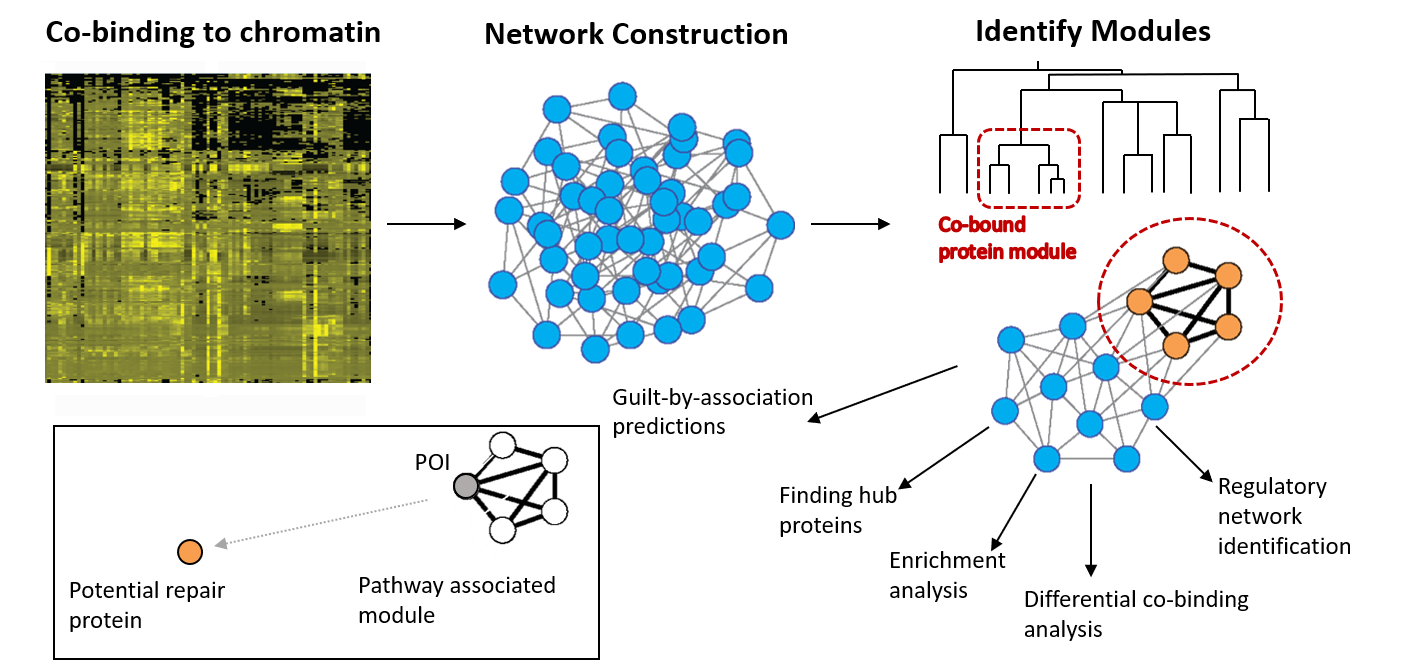
\includegraphics[width=.98\textwidth]{resources/images/Intro/co-expression.png}
    \caption[Schematic of co-binding analysis]{\textbf{Schematic of co-binding analysis. }Schematic of the steps used in co-binding analysis. Pairwise correlation is used to determine the relationship between each possible pair. This is followed by filtering of said relationships in alignment with appropriate thresholds and the visualization the remaining correlation values in form of a network. This network is then used to identify functional modules using grouping methods such as hierarchical clustering. From these modules hubs and regulating factors as well as functional predictions can be drawn. The latter can be based on the "Guilt-by-association" approach (GBA, highlighted) that identifies the function of unknown variables by the variables they cluster with. Gene co-binding is generally mathematically analogous to the protein co-regulation studied in this thesis.\\\cite{vanDam.2018}, modified}
    \label{fig:co-expression}
\end{figure}
With the created network tables using TOM as a measure of the similarity between chromatin binding behavior of repair and replication proteins it is now possible to apply clustering algorithms such as Diffusion based Network Propagation to identify functional DNA repair modules for all sets and for each DNA lesion individually. To ensure that a maximum amount of data is available to the Nearest Neighbor- and Diffusion clustering algorithms we calculated TOM maps for all DNA lesion sets including all proteins found in each run ($N_{max}=4313$). Those edge lists are only available to the clustering algorithms and can not be plotted as networks on the DRA itself. Scale-freeness for these networks was analyzed as explained above and can the corresponding plots can be seen in the supplementary collection on Github.


\subsection{Using TOM networks and Diffusion clustering to identify functional modules}
In addition to the previously included reference network consisting of 295 known DNA repair and replication proteins we now included DNA lesion specific repair networks based on topological overlap measures for DNA-Protein Crosslinks (DOC), Doublestrand Breaks (DSB), Interstrand Crosslinks (ICL), Replication Fork Collapse (FC) as well as a network visualizing protein involvement in Replication Termination (RT). These networks can be visualized using the JavaScript package cytoscape.js on demand including only the 1737 most abundant proteins under damage conditions. In addition to the processing steps mentioned in Section \ref{sec:netprocessing} a soft threshold for plotting is applied to the raw edge list before plotting. The back-end is configured in such a way that it only plots edges that have a weight higher than $0.7 * EdgeWeight_{max}$ to improve plotting performance.\\
When visualizing the networks one has to consider that each network is based on a specific set of experiments using different methods, DNA templates and especially treatments that can greatly influence the appearance and accessibility of a network plot itself. We've already mentioned that not all of the unfiltered networks can follow the scale free principle. Especially networks created from a small list of conditions and that therefore had less information available to the correlation- and TOM algorithms are very interconnected. Even though all our networks fit our criteria for biological scale free-like networks we see large differences in the plotted filtered networks (see Figures \ref{fig:DPCtom} through \ref{fig:RTtom}) with especially the ICL and DPC networks being relatively inaccessible to the users naked eye. We defined accessibility of a network as the ability of a trained user to distinguish groups of functionally similar proteins in the network plot solely by means of observation.\\ Before starting to mine the constructed networks for functional protein modules we determined that the algorithm parameters should be set to $iter = 1000000$ and $reset = 0.25$ while the number of proteins to be plotted after diffusion varies for each query. These parameters gave us results representing known modules with a great balance between computation time and accuracy.


\subsubsection{Analysis of the DNA-Protein Crosslink Network}
\label{sec:dpcnet}
\begin{figure}[H]
    \centering
    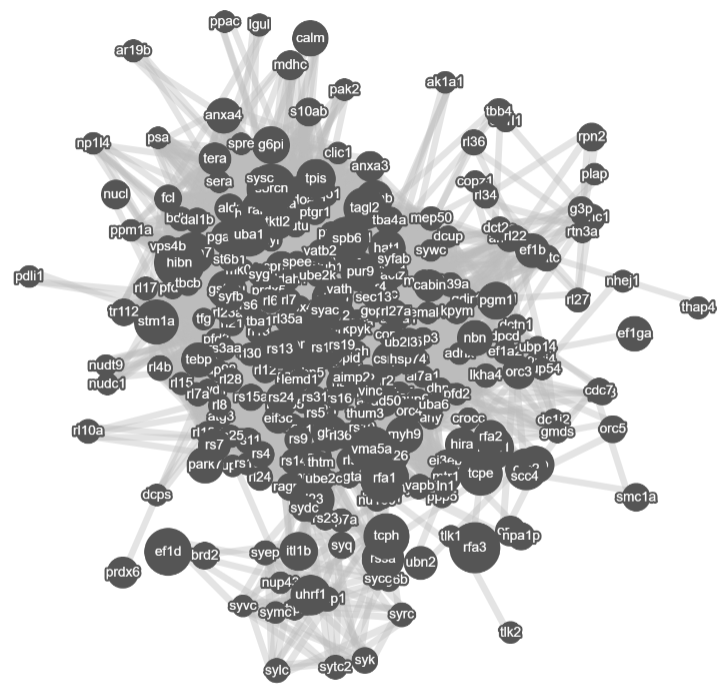
\includegraphics[width=.6\textwidth]{resources/images/Results/DPC_networkplot.png}
    \caption[DNA-Protein Crosslink TOM Network]{\textbf{DNA-Protein Crosslink TOM Network. }Depicted is the visual representation of proteins loaded onto chromatin under DNA-Protein Crosslink conditions. Edges are filtered using a soft threshold of 70\% and their width  is proportional to their score. Node size represents the protein enrichment scores.}
    \label{fig:DPCtom}
\end{figure}
As mentioned in the introduction of this work DNA-Protein Crosslinks are mostly repaired in a replication dependent manner through mechanisms that are mediated by the proteasome and the metalloprotease SPRTN. Using the network shown in Figure \ref{fig:DPCtom} one can observe replication factors on the outer right and bottom parts of the network as well as many subunits of the proteasome in the center that are grouped together. Due to the soft threshold applied for plotting SPRTN is not included in the network plot but is still available for the diffusion algorithm. To investigate whether the unfiltered network used for clustering represents published protein interactions and DNA binding mechanisms in DNA-Protein Crosslink repair we used SPRTN, PCNA and the MCM helicase as a query for the diffusion algorithm. Plotting the 20 best results yielded us the cluster shown in \ref{fig:sprtn_cluster}.\\
\begin{figure}[H]
    \centering
    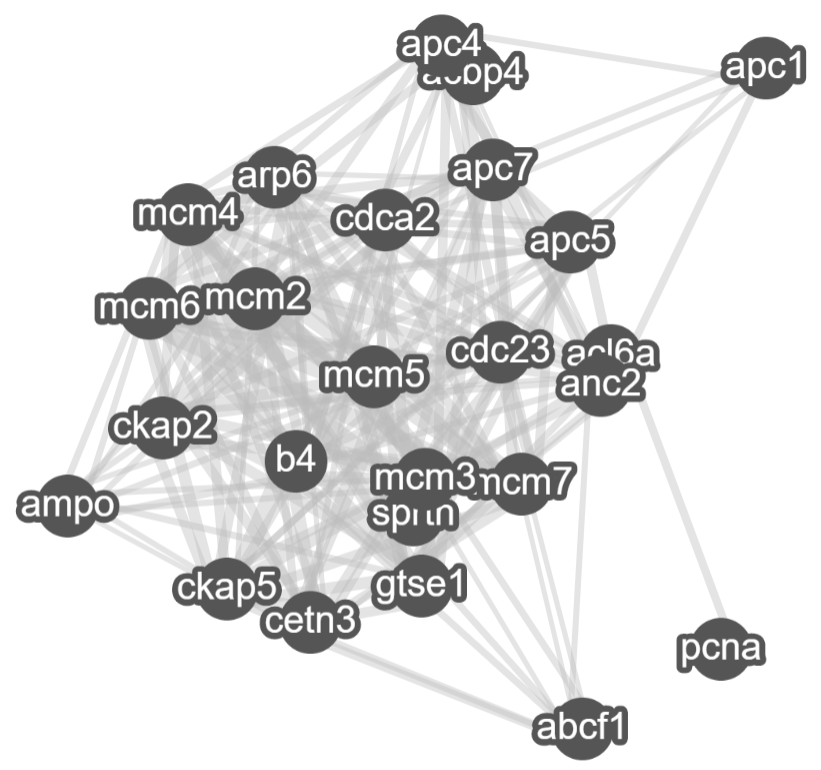
\includegraphics[width=0.5\textwidth]{resources/images/Results/sprtn_mcm_pcna_diffusion.PNG}
    \caption[Diffusion result for SPRTN and repliation associated proteins under DPC conditions]{\textbf{Diffusion result for SPRTN and repliation associated proteins under DPC conditions. }Shown is the resulting cluster graph of the diffusion algorithm based on the unfiltered DPC network.\\Query: SPRTN, PCNA, MCM2-7; 20 nodes}
    \label{fig:sprtn_cluster}
\end{figure}
This diffusion output validated that the subunits of the MCM helicase have a high similarity over all conditions of the DPC experiment series. Additionally, they seem to have a highly similar chromatin binding profile to PCNA and other DNA replication factors and checkpoint proteins such as CDC23 and CDCA2. Interestingly there is no direct edge between PCNA and SPRTN despite \cite{Vaz.2016} showing that SPRTN binds directly to the replication fork where PCNA is always loaded during replication. 
This could be an artifact of the experimental setup which relied on only two time points for the untreated control whereas five time points were measured under DNA-Protein Crosslink conditions. These differences in the setup between each condition can, as mentioned, heavily influence the performance of similarity measures such as TOM due to the fact that the correlation matrix those measures are based on make the assumption of equally distributed observations over all conditions which was not the case here.\\
Also noticeable is the lack of the SPRTN interactor p97, an ATPase that forms a dimer with Cdc48p and is involved in DPC repair \citep{Larsen.2019,Woodman.2003}. 
\begin{figure}[H]
    \centering
    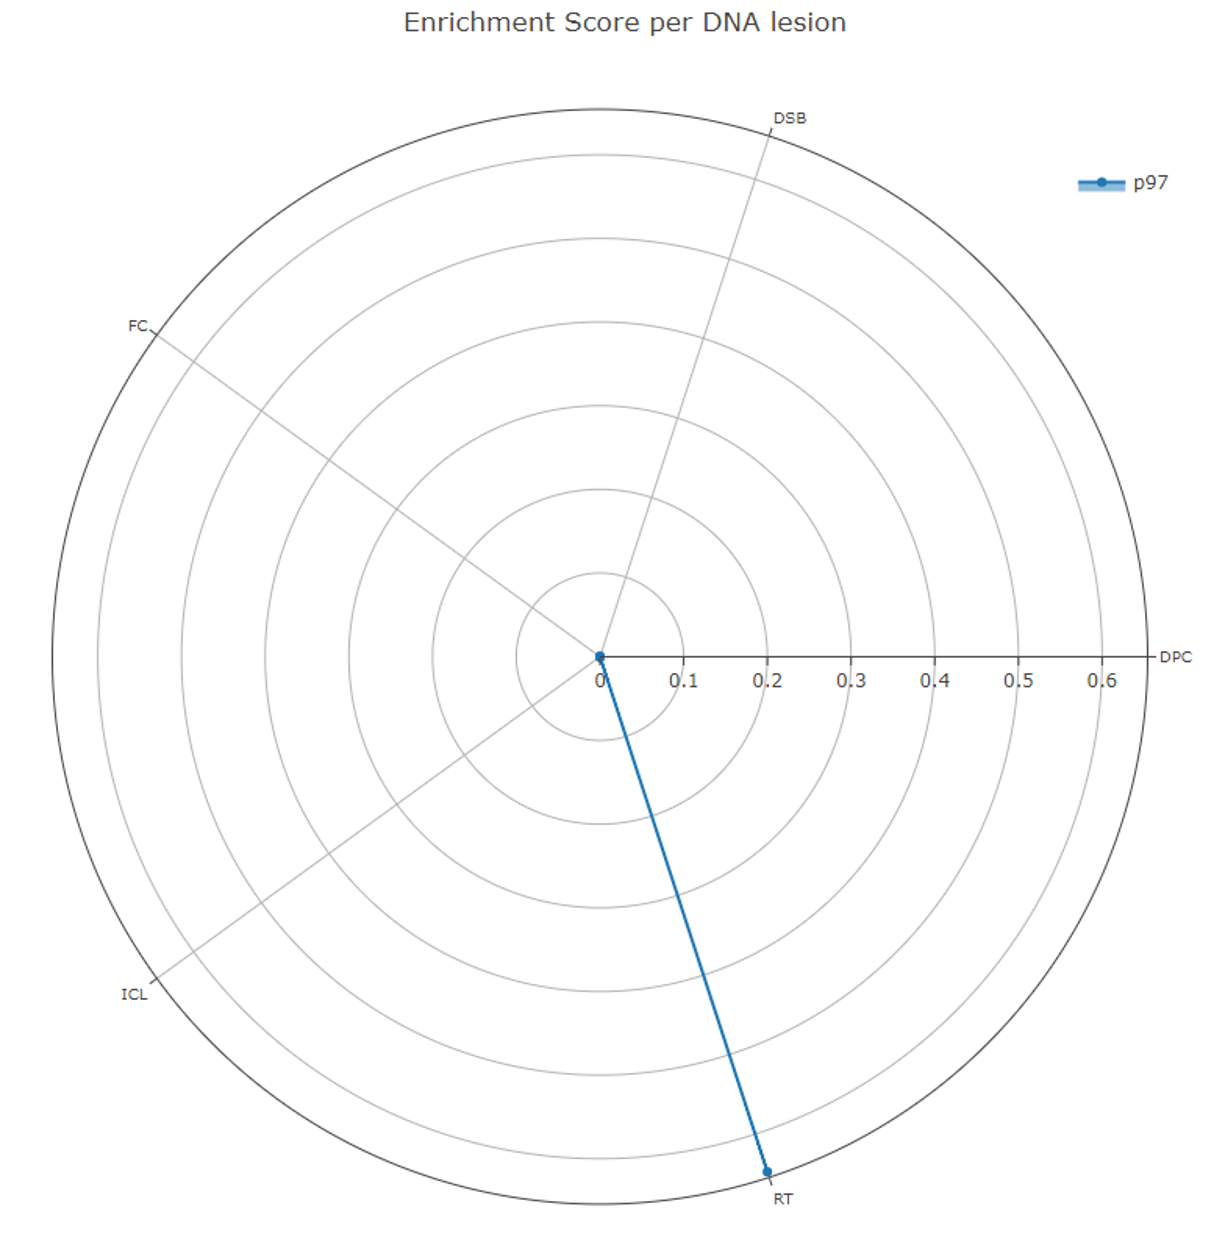
\includegraphics[width=.5\textwidth]{resources/images/Results/p97_enrichment.png}
    \caption[Enrichment of p97 over all DNA lesion types]{\textbf{Enrichment of p97 over all DNA lesion types. }Shown are the enrichment scores for p97 over all DNA lesion types. p97 only has a score for Replication Termination suggesting it has not been measured in any other set in a significant abundance.}
    \label{fig:p97dpc}
\end{figure}
Digging deeper through the data one can find that p97 has not been detected in the sets used to create the DSB network (see Figure \ref{fig:p97dpc}) which can be expected given the use of pure non-replicating HSS. p97 should be only introduced to the system once NPE is added.


\subsubsection{Analysis of the Doublestrand Break Network}
\label{sec:dsbnet}
\begin{figure}[H]
    \centering
    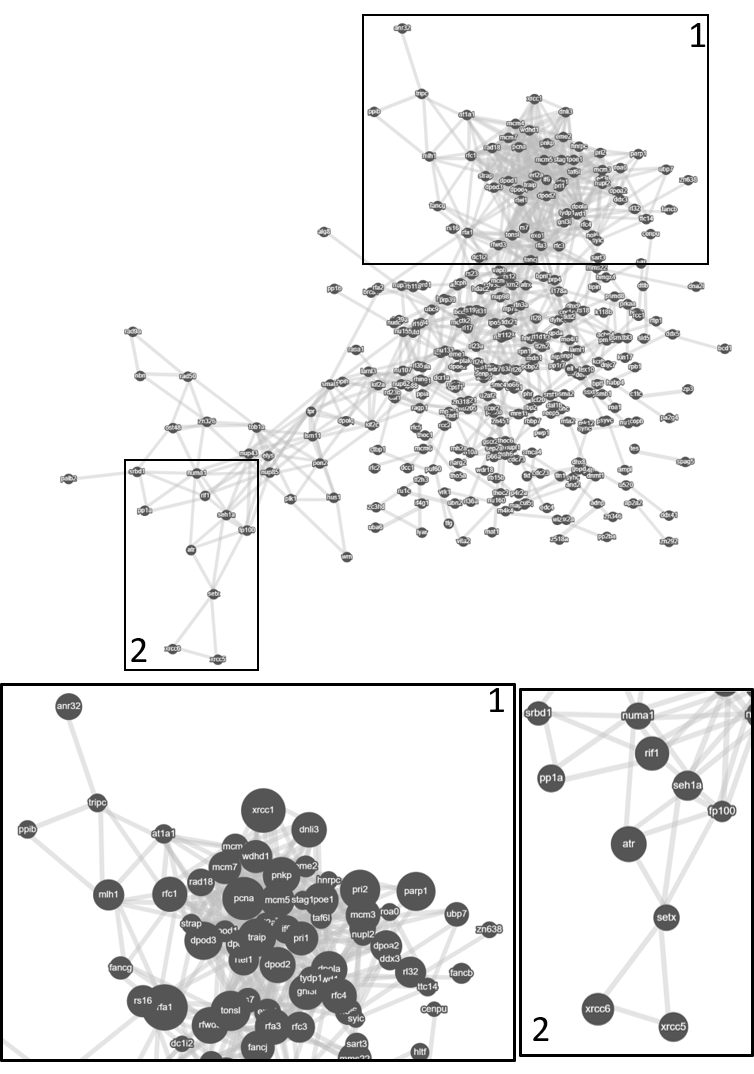
\includegraphics[width=.8\textwidth]{resources/images/Results/DSB_networkplot.png}
    \caption[Doublestreand Break TOM Network]{\textbf{Doublestreand Break TOM Network. }Visual representation of proteins loaded onto chromatin under Doublestrand Break conditions. Edges are filtered using a soft threshold of 70\% and their width  is proportional to their score. Node size in zoomed windows represents the protein enrichment scores.}
    \label{fig:DSBtom}
\end{figure}
In contrast to all other networks looked at in this work the DSB network used experiment sets only collected using HSS meaning that this network depicts replication independent DSB repair. Proteins associated with replication initiation and origin licensing will be found in the set but replication firing could not occur. As can be seen in Figure \ref{fig:DSBtom} the Doublestrand Break network shows groups of proteins that are distinguishable by means of observation. The network itself feature a low number of nodes with diverse degrees. Looking at the top right (labeled \textbf{1}) group of proteins one can make out proteins associated with origin licensing (Section \ref{sec:cellcycle}) and the formation of a pre-RC as well as the first polymerases with missing co-factors. Additionally, the E3 ubuquitin ligase TRAIP is closely connected to PCNA indicating the successful detection of DNA damage. In the bottom left of the network another high scoring group of proteins including ATR and the DSB repair factors XRCC5 and XRCC6 can be seen. This network represents mechanisms of DSB repair fairly well even in its filtered form for plotting. To see whether full DSB repair modules can be identified we used the known repair factors ATR, ATM, TRAIP, XRCC5 and XRCC6 as the query for our diffusion algorithm and plotted the 30 highest scoring proteins in Figure \ref{fig:atratm_diff}.
\begin{wrapfigure}{r}{0.5\textwidth}
    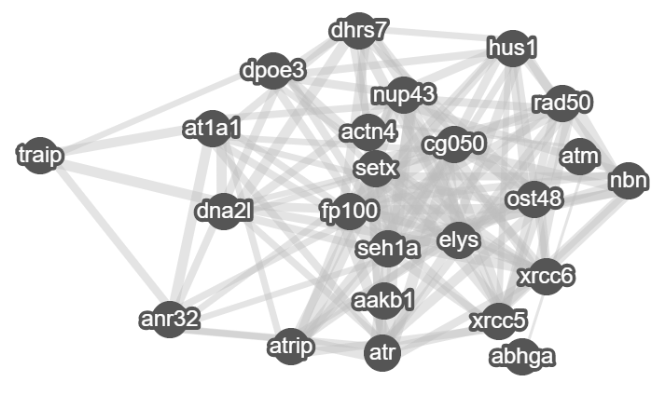
\includegraphics[width=0.46\textwidth]{resources/images/Results/dsb_diff_atratm.PNG}
    \caption[Diffusion result for ATR, ATM and other DSB repair proteins under DSB conditions]{\textbf{Diffusion result for ATR, ATM and other DSB repair proteins under DSB conditions. }Shown is the resulting cluster graph of the diffusion algorithm based on the unfiltered DSB network.\\Query: ATR, ATM, TRAIP, XRCC5, XRCC6; 30 nodes}
    \label{fig:atratm_diff}
\end{wrapfigure}
As \cite{Cimprich.2008} showed in their review on the function ATR in maintaining genome integrity the replication independent repair of DSBs works in two ways. The first mechanisms detects ssDNA by RPA binding which in turn leads to ATR/ATRIP recruitment as well as the loading of the 9-1-1 complex (Rad9-Hus1-Rad1) onto the first available dsDNA section after the DSB. This method is reflected in the lower part of the cluster seen on the right. The right side of the cluster represents the detection and repair of double stranded ends via ATM and the following recruitment of RAD50.\\
To further show how robust the DSB network is in representing protein recruitment profiles we used the MCM helicase subunits MCM2-7 as an input for Diffusion and plotted the 15 highest scoring proteins the result of which can be seen in Figure \ref{fig:diff_mcm_dsb}. It shows a closed cluster of all MCM subunits as well as the DNA polymerases (Pol\textdelta~ and Pol\textalpha) expected on licensed chromatin. Additionally the SMC5/6 loading factor Slf1  (as ANR32; \cite{Raschle.2015}) is depicted as behaving similar to MCM4, 5 and 7 as well as Pol\textdelta~ subunit 1. 
\begin{figure}
    \centering
    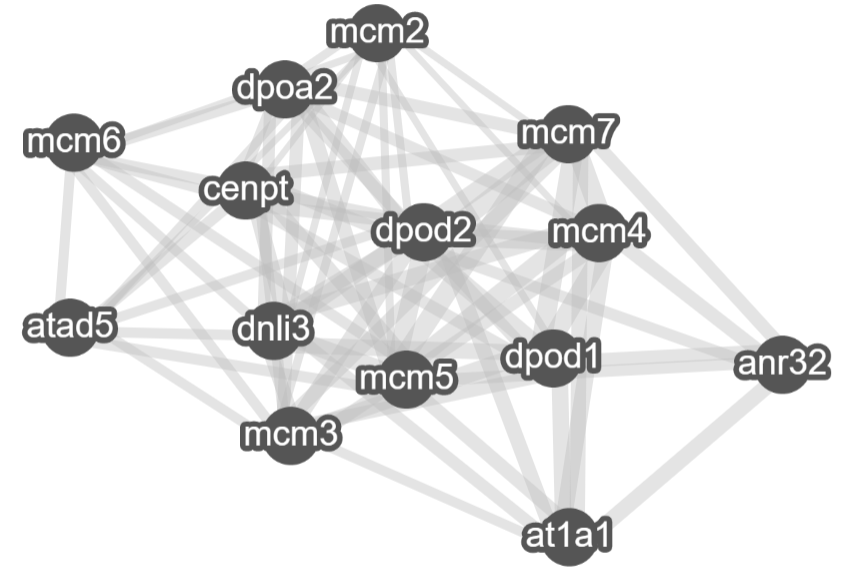
\includegraphics[width=.5\textwidth]{resources/images/Results/diff_mcm_dsb.PNG}
    \caption[Diffusion result for the MCM helicase]{\textbf{Diffusion result for the MCM helicase. }Shown is the resulting cluster graph of the diffusion algorithm based on the unfiltered DSB network.\\Query: MCM2-7; 15 nodes}
    \label{fig:diff_mcm_dsb}
\end{figure}
This result suggests that the newly deployed DSB TOM network represents the recruitment of DSB repair proteins as well as the processes of chromatin licensing and the formation of the pre-RC in non-replicating extracts.\newpage
\subsubsection{Analysis of the Replication Fork Collapse network}
\begin{figure}[H]
    \centering
    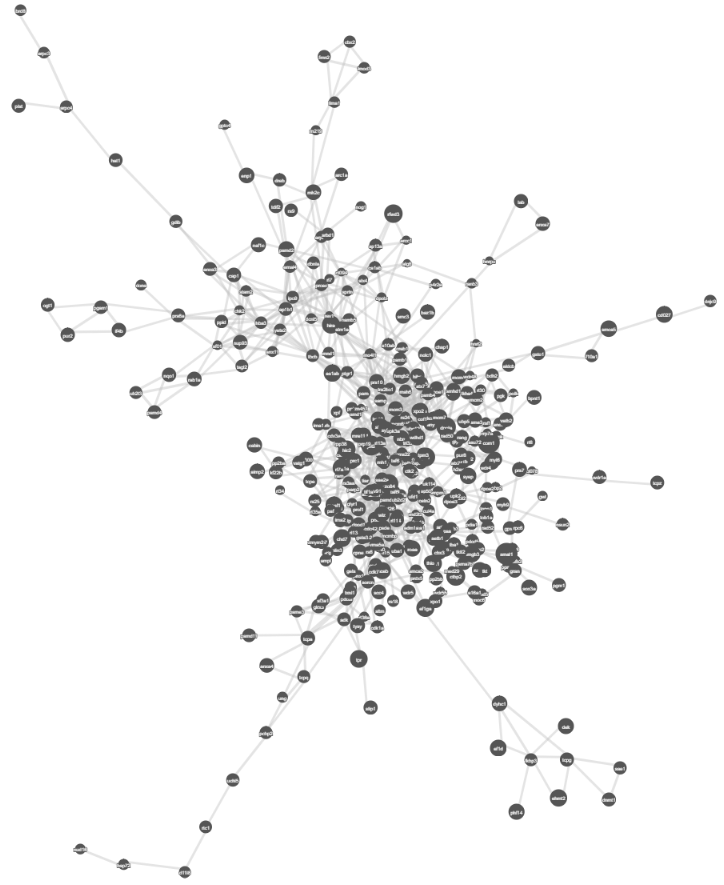
\includegraphics[width=.8\textwidth]{resources/images/Results/FC_networkplot.png}
    \caption[Fork Collapse TOM Network]{\textbf{Fork Collapse TOM Network. }Visual representation of proteins loaded onto chromatin during Replication Fork Collapse. Edges are filtered using a soft threshold of 70\% and their width  is proportional to their score. Node size in zoomed windows represents the protein enrichment scores.}
    \label{fig:FCtom}
\end{figure}
During the replication of DNA the replisome encounters many obstacles such as DNA damages or sequences that are difficult to replicate. These obstacles can cause fork stalling that may lead to the collapse of the fork itself by replisome disassembly. In his review \cite{Cortez.2015} describes how the replication checkpoint prevents replication fork stalling for example via the regulation of helicases like BLM, nucleases like DNA2 and EXO1 and translocases like SMARCAL1 via ATR.
All of the mentioned enzymes fulfill roles in different repair mechanisms but all have in common that they are involved in fork regression or fork reversal (see Section. \ref{sec:polblock}). The result of using these enzymes as a query to diffuse over the unfiltered Fork Collapse network can be seen in Figure \ref{fig:atrtarget_diff_fc}.
\begin{wrapfigure}{r}{0.5\textwidth}
    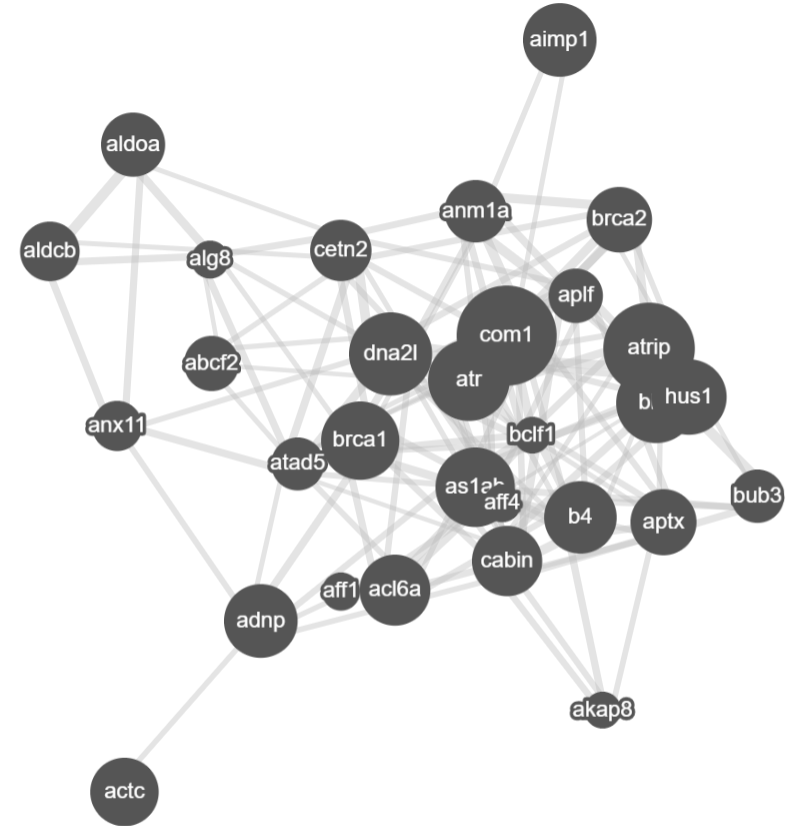
\includegraphics[width=0.46\textwidth]{resources/images/Results/fc_atrtargets.PNG}
    \caption[Diffusion result for ATR, BLM, DNA2 and SMARCAL1 under Fork Collapse conditions]{\textbf{Diffusion result for ATR, BLM, DNA2 and SMARCAL1 under Fork Collapse conditions. }Shown is the resulting cluster graph of the diffusion algorithm based on the unfiltered DSB network.\\Query: ATR, BLM, DNA2(DNA2L), SMARCAL1 (HUS1); 30 nodes}
    \label{fig:atrtarget_diff_fc}
\end{wrapfigure}
The highest node with the highest diffusion score within the resulting cluster is ATR indicating that it connects most of the found nodes with another and therefore could play a crucial role in their recruitment or function. As is already known, direct targets of ATR are involved in fork reversal suggesting that the FC-TOM network represents the mechanism of fork collapse well. On the right side of the cluster one can see the translocase HUS1 (SMARCAL1) in close vicinity to the helicase BLM and ATRIP, the ATR interacting protein. These targets of ATR are closely connected to the high scoring repair proteins BRCA1, BRCA2 and APTX (XRCC1) that were also present and enriched in experiments investigating the replication-independent repair of DSBs (see Section \ref{sec:dsbnet}). Given the fact that double- and singlestrand breaks are a common cause of replication fork stalling and also a result of proteasome dissociation \citep{Cortez.2015} the inclusion and high diffusion- and enrichment scores for these factors is expected. 



\subsubsection{Analysis of the Interstrand Crosslink network}
\label{sec:iclnet}
The Interstrand Crosslink network is built on the person correlation based TOM of NPE/HSS using Psoralen-treated sperm chromatin. Under Psoralen treatment interstrand crosslinks are introduced at random into the chromatin template and mostly repaired via the Fanconi Anemia (FA) pathway. The mechanism of ICL bypass and repair in \textit{Xenopus} egg extracts has been resolved in high detail by \cite{Raschle.2015}. Replication of Psoralen-treated chromatin starts with the loading of all necessary replication proteins followed by triggering a transient checkpoint response. After encountering an ICL replicative DNA polymerases are unloaded while TLS polymerases as well as the entire Fanconi core complex are loaded. Additionally the nucleases XPX and FAN1 are loaded together with the FA core complex that is loaded by a ubiquitylated FANCD2/FANCI dimer \citep{Raschle.2015,Knipscheer.2009,Raschle.2008}.
\begin{figure}[H]
    \centering
    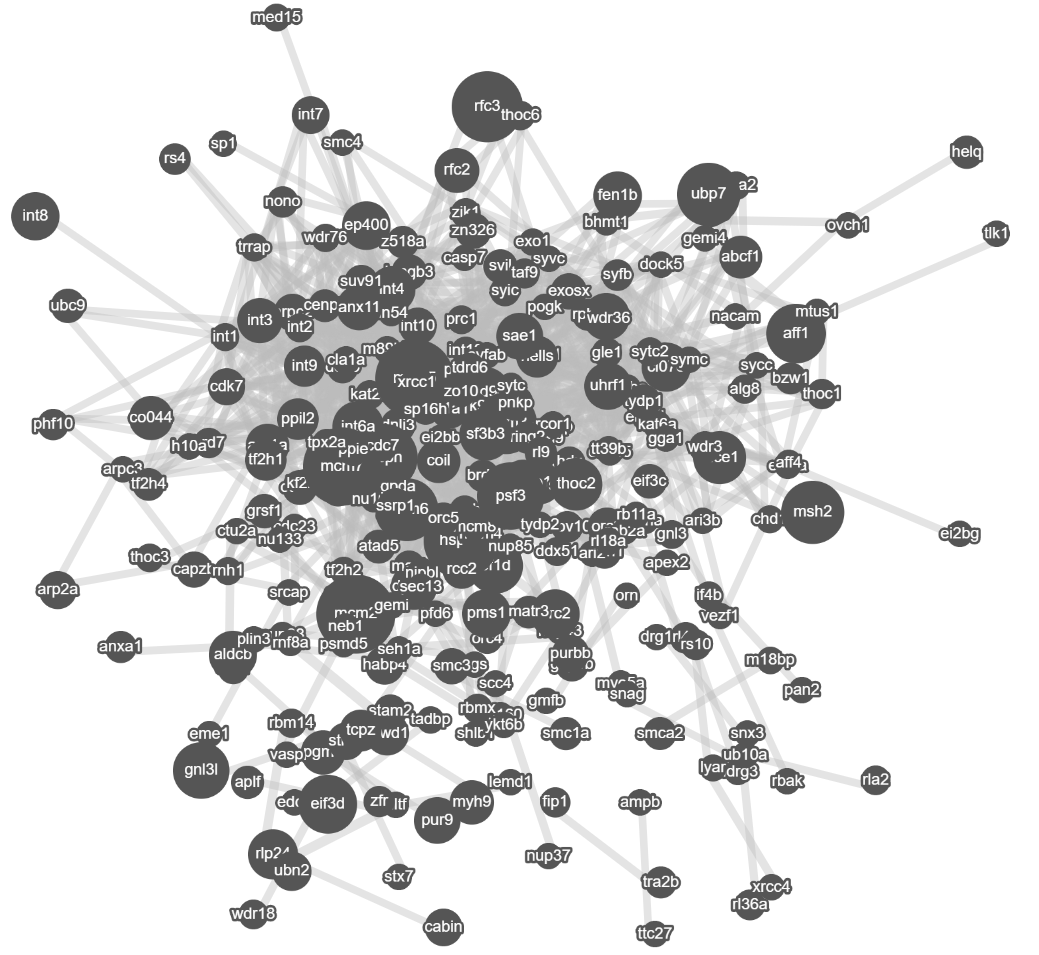
\includegraphics[width=\textwidth]{resources/images/Results/ICL_networkplot.PNG}
    \caption[Interstrand Crosslink TOM Network]{\textbf{Interstrand Crosslink TOM Network. }Visual representation of proteins loaded onto chromatin under Interstrand Crosslink conditions. Edges are filtered using a soft threshold of 70\% and their width  is proportional to their score. Node size in zoomed windows represents the protein enrichment scores.}
    \label{fig:ICLtom}
\end{figure}
Using the FA core complex as the query to diffuse over the ICL network we expected to find most repair enzymes as well as TLS polymerases in the resulting cluster.
\begin{wrapfigure}{l}{0.5\textwidth}
    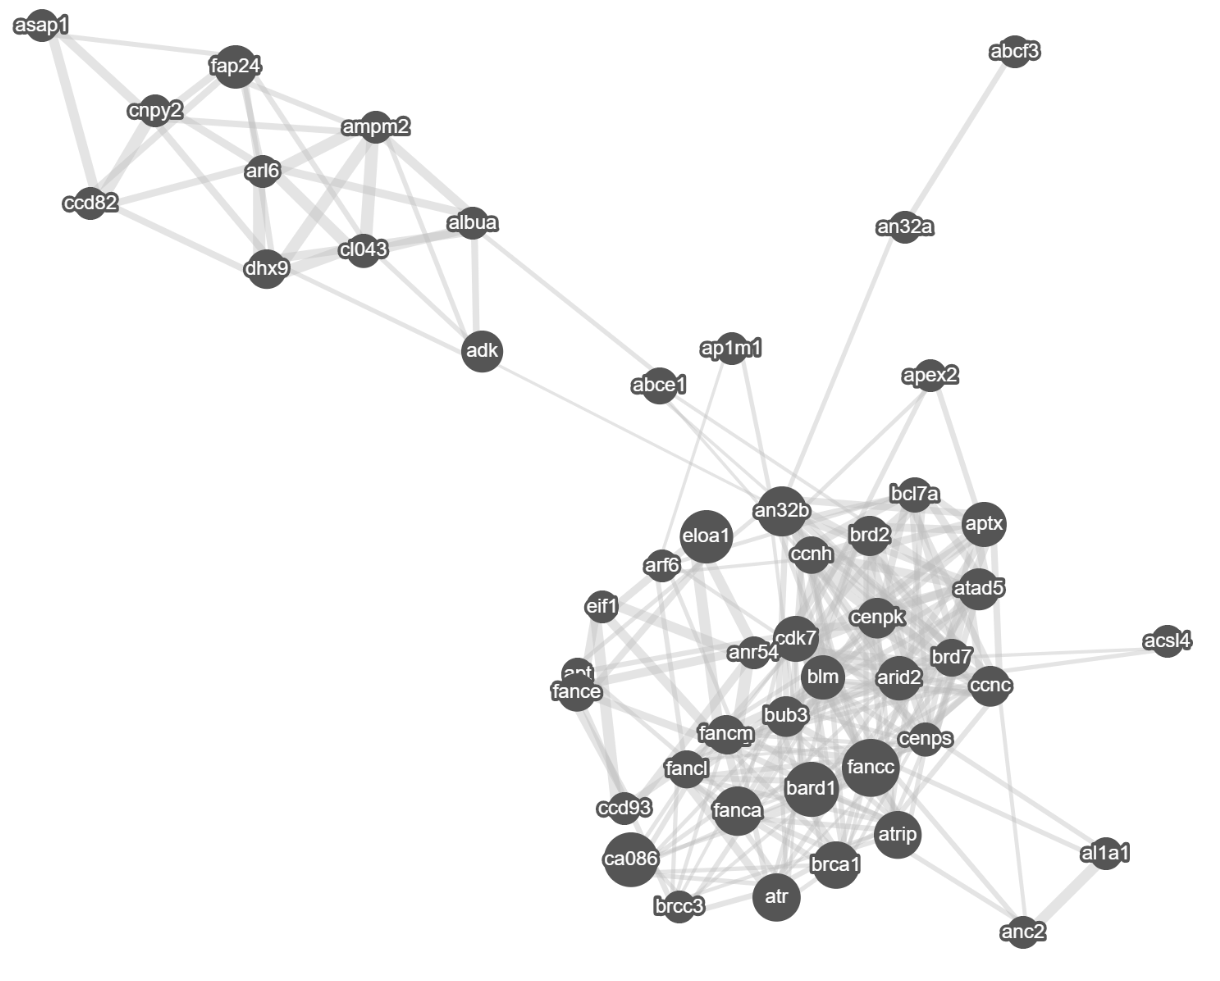
\includegraphics[width=0.46\textwidth]{resources/images/Results/FAcore_diff_ICL_50.PNG}
    \caption[Diffusion result for the Fanconi core complex under Interstrand Crosslink conditions]{\textbf{Diffusion result for the Fanconi core complex under Interstrand Crosslink conditions. }Shown is the resulting cluster graph of the diffusion algorithm based on the unfiltered DSB network.\\Query: GO:0043240; 50 nodes}
    \label{fig:atrtarget_diff_fc}
\end{wrapfigure}
Surprisingly, of the FA loading complex dimer only FANCI could be detected. Otherwise all proteins of the FA core complex are closely connected to the helicase BLM as well as ATR and BRCC3. The latter is a subunit of an E3 ubiquitin ligase which is involved in the recruitment of BRCA1 to DNA lesions. BRCA1 is also found in the resulting cluster being a direct neighbor to FANCC and FANCA as well as ATRIP and ATR. Given the slightly shifted peaks of FA and its recruiters as well as the TLS polymerases and FA itself it is possible that the proteins expected to be included in the first cluster are not in the list of 50 highest scoring neighbor nodes we defined. Outputting a cluster consisting of 100 nodes for example will not be plotted because the server takes to long to answer the users request and the script runs into a hard coded timeout that can not be changed.\\
To circumvent this problem we repeated the diffusion using the FA recruiter FANCD2 and POL\textkappa, a TLS polymerase, as the query proteins and plotting the 50 highest scoring proteins. Approaching the search for ICL repair related proteins from the angle of known regulatory proteins resulted in the expected group of proteins. 
\begin{figure}[H]
    \centering
    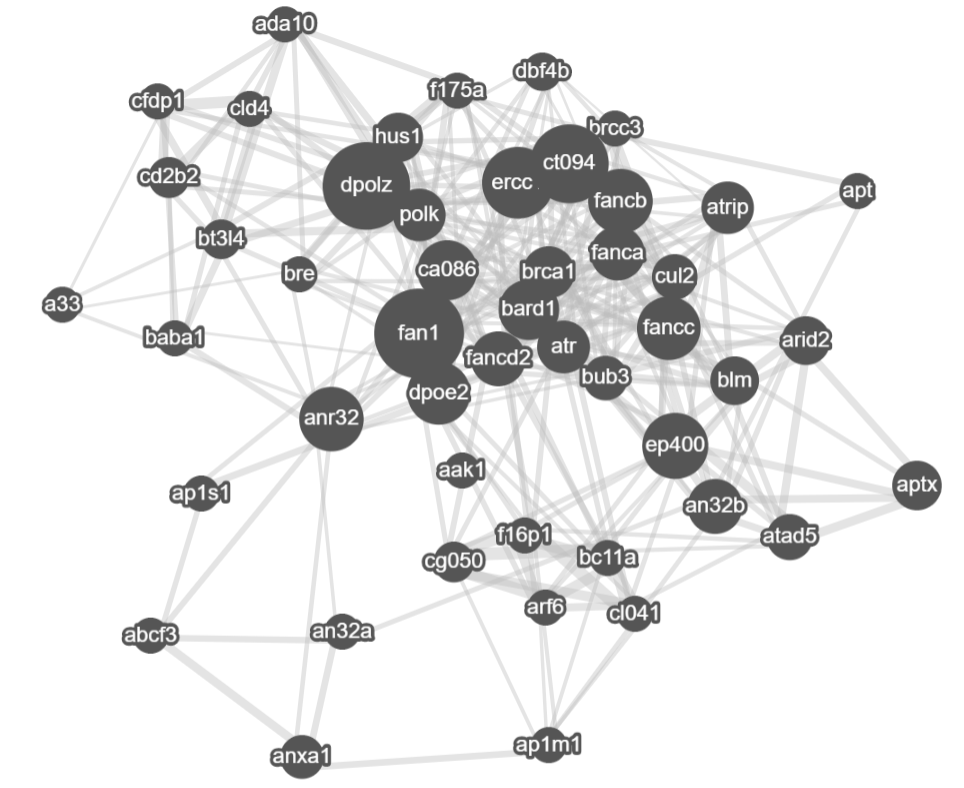
\includegraphics[width=0.5\textwidth]{resources/images/Results/icl_diff_fancd2_polk.PNG}
    \caption[Diffusion result for FANCD2 and POL\textkappa~ under Interstrand Crosslink conditions]{\textbf{Diffusion result for the Fanconi core complex and its recruiters under Interstrand Crosslink conditions. }Shown is the resulting cluster graph of the diffusion algorithm based on the unfiltered DSB network.\\Query: FANCD2, POL\textkappa; 50 nodes}
    \label{fig:icl_diff_fancd2_polk}
\end{figure}
Using FANCD2 and POL\textkappa~ to diffuse over the ICL network yielded a cluster of highly enriched enzymes known to be involved in ICL repair. Aside from the DNA binding subunits of the FA core complex (FANCA and FANCB) the repair associated helicase BLM was found in direct neighborhood of FANCC together with ATR and BRCA1 as it was the case for the diffused cluster using the FA core complex. Other enzymes involved in doublestrand break repair such as HUS1 and ATRIP are also part of the cluster which is to be expected considering that it is possible for ICLs to be bypassed using a combination of translesion synthesis and doublestrand break repair (see Section \ref{sec:iclrepair} for details). Another highly enriched protein included in the cluster is FAN1 which is a nuclease found to be associated with the FA core complex and FANCD2 thought to act together with MUS81 cut covalently crosslinked DNA \citep{ODonnell.2010}. Another interesting protein in the cluster is DPOLZ (also known as REV3), the catalytic subunit of DNA polymerase zeta. It is known to be involved in DNA repair, especially in the replication-dependent resolution of doublestrand breaks and therefore it plays a major role in bypassing covalent ICLs \citep{Raschle.2008} as REV3 depleted \textit{Xenopus} egg extracts have been shown to be ICL repair deficient \citep{Raschle.2008}.

\subsubsection{Analysis of the Replication Termination network}
\begin{figure}[H]
    \centering
    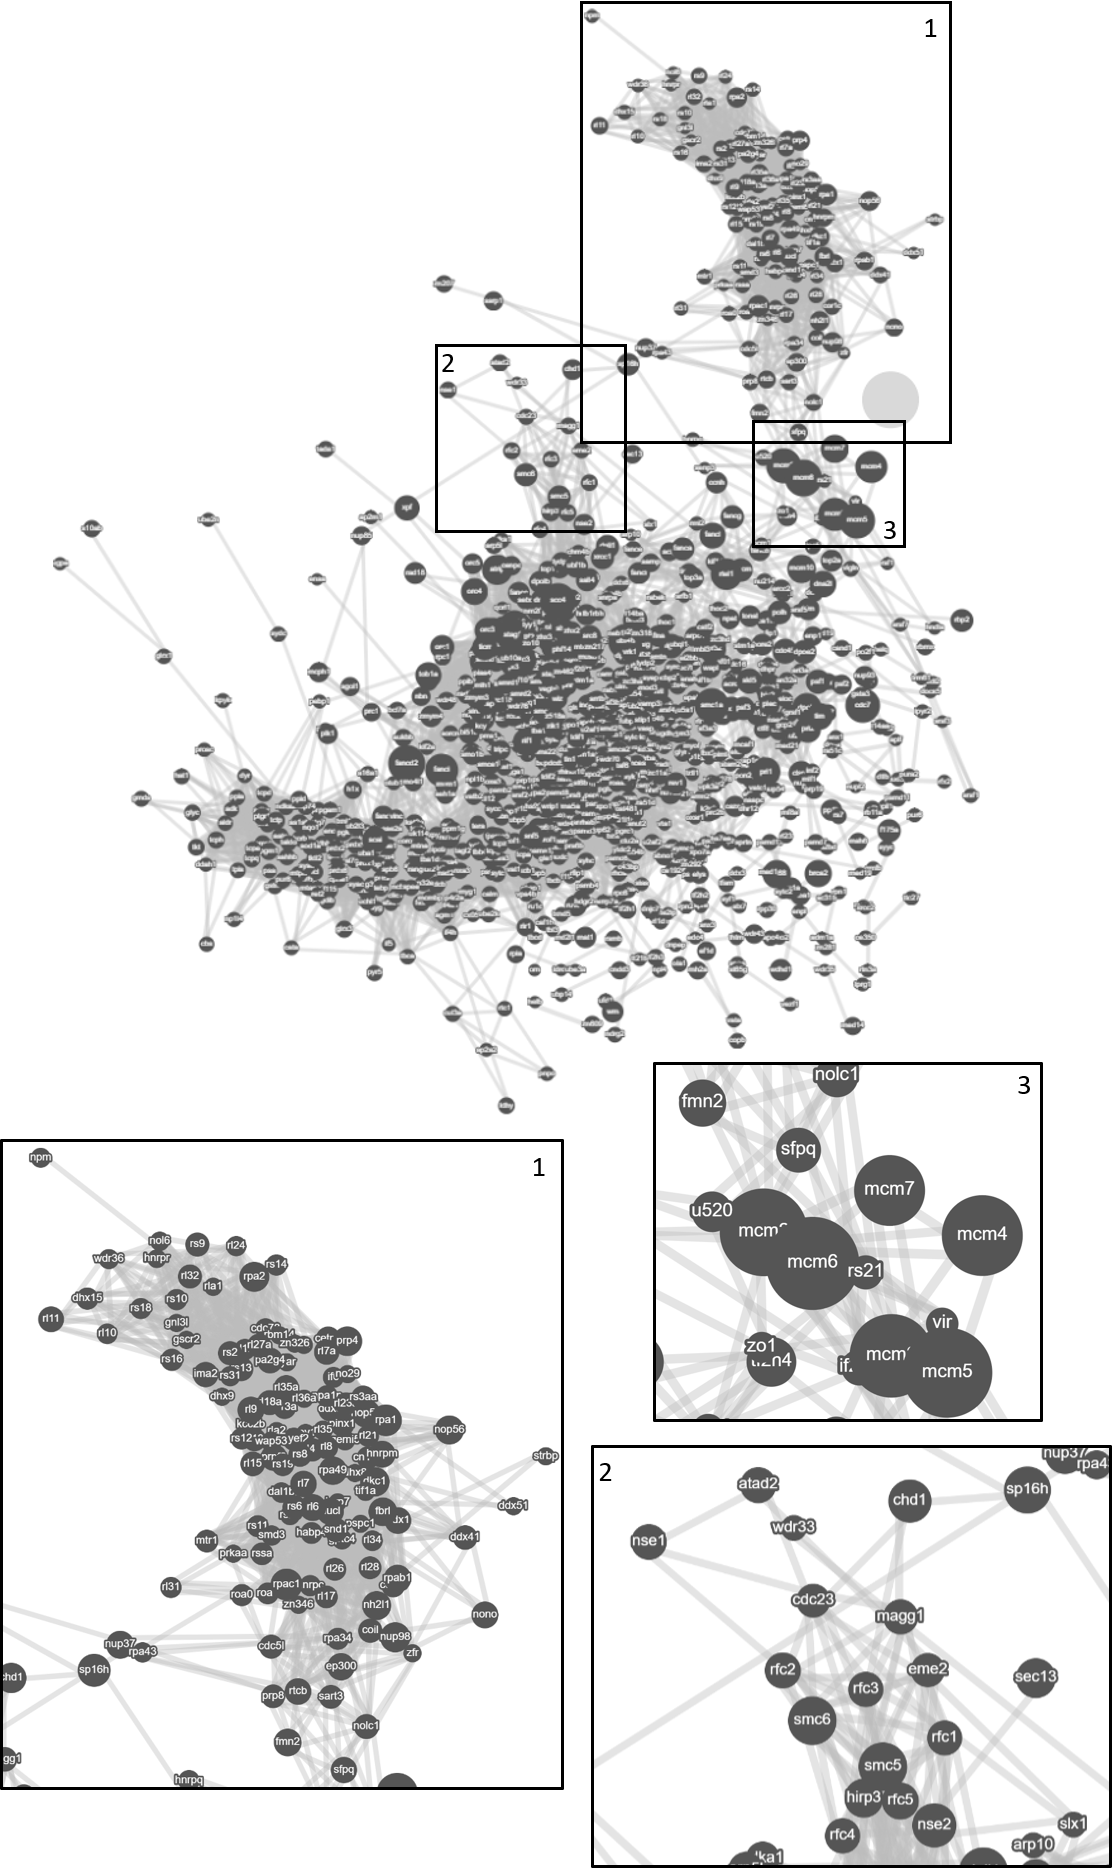
\includegraphics[width=.7\textwidth]{resources/images/Results/RT_networkplot.png}
    \caption[Replication Termination TOM Network]{\textbf{Replication Termination TOM Network}. Visual representation of proteins loaded onto chromatin during Replication Termination. Edges are filtered using a soft threshold of 70\% and their width  is proportional to their score. Node size in zoomed windows represents the protein enrichment scores.}
    \label{fig:RTtom}
\end{figure}

\subsection{The benefits of using individual damage networks over combined network representation}

